\documentclass[a4paper, 12pt]{article}
% math symbols
\usepackage{amssymb}
\usepackage{amsmath}
\usepackage{mathrsfs}
\usepackage[shortlabels]{enumitem}
\usepackage{mathseries}
\usepackage[12pt]{moresize}
\usepackage[style = alphabetic, maxbibnames = 99, backend = biber]{biblatex}
\addbibresource{references.bib}

\usepackage[margin = 2cm]{geometry}

\tolerance = 1000
\emergencystretch = 0.74cm



\pagestyle{empty}
%\parindent = 0mm


\setmathstyle{2020}{Теория информации}{С.А. Лучинин, М.С. Опанасенко}


\newtheorem{problem}{Задача}[section]
\newtheorem{examples}{Задача}[section]
\makeatletter
\renewtcolorbox[use counter = theorem, number within = section]{problem}[1][]{
    enhanced,
    theo = {blue},
    title = {Задача \thetcbcounter\ #1},
    before upper = {\protected@edef\@currentlabel{\csname p@theorem\endcsname\csname thetcbcounter\endcsname}}
}
\makeatother
\makeatletter
\renewtcolorbox[use counter = theorem, number within = section]{examples}[1][]{
    enhanced,
    theo = {blue},
    title = {Пример \thetcbcounter\ #1},
    before upper = {\protected@edef\@currentlabel{\csname p@theorem\endcsname\csname thetcbcounter\endcsname}}
}
\makeatother


%\let\M\undefined
\let\IP\undefined
\newlang{\IP}{\lang{IP}}

\newauthor{ds}{Dmitry}{red!20}

\begin{document}
    \pagestyle{empty}


\begin{tikzpicture}[remember picture, overlay]
    \node[
        shape = rectangle,
        minimum height = \paperheight,
        minimum width = \paperwidth,
        anchor = south west,
        fill = olive!5]
        (sheet) at (current page.south west) {};
    \tikzset{shift = {(sheet.center)}}
    \node at (0, -2) {
        \HUGE
        \begin{tabular}{c}
            \textsc{Теория информации}\\
            \huge Конспект лекций
        \end{tabular}
    };

    \node[inner sep = 0pt, opacity = 0.5] at (6, 10.5){
        
\includegraphics[width = 0.27\textwidth] {pics/sun.png}
    };


    \begin{scope}[shift = {(0, 3)}]
        \node[inner sep = 0pt, opacity = 0.5] at (-5, 0){
            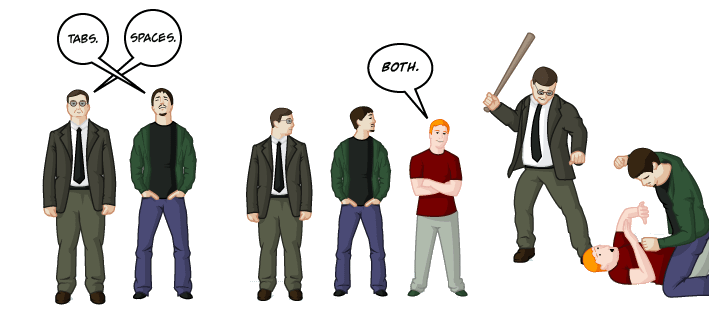
\includegraphics[width = 0.4\textwidth] {pics/tabs-spaces.png}
        };
        \node[inner sep = 0pt, opacity = 0.5] at (-5, -2.3){
            \textsc{Коммуникационная сложность}
        };
        \node[inner sep = 0pt, opacity = 0.5] at (5, 0){
            
\includegraphics[width = 0.4\textwidth] {pics/bender.png}
        };
        \node[inner sep = 0pt, opacity = 0.5] at (5, -2.3){
            \textsc{Колмогоровская сложность}
        };
    \end{scope}

    \begin{scope}[shift = {(0, -8)}]
        \node[inner sep = 0pt, opacity = 0.5] at (0, 0){
            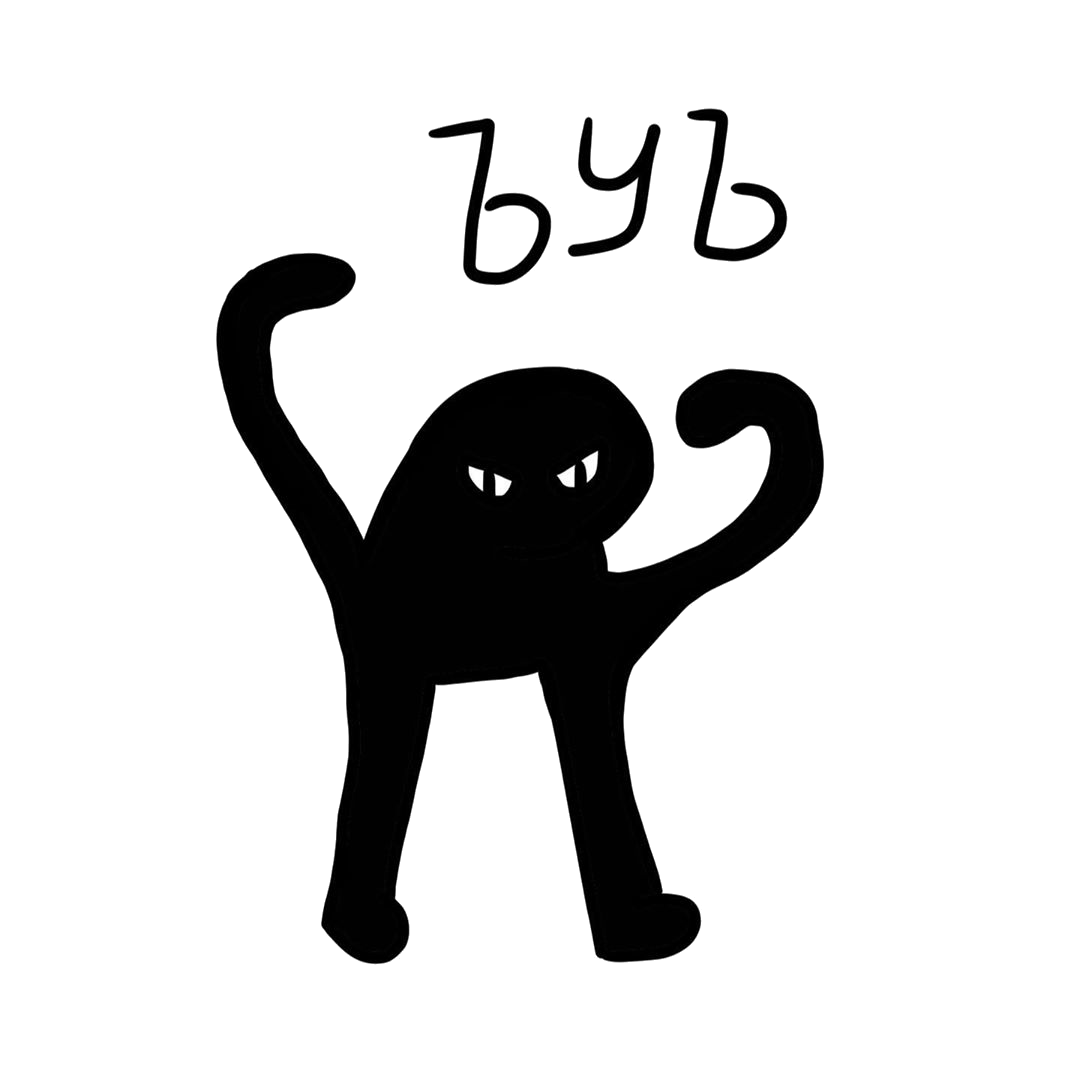
\includegraphics[width = 0.5\textwidth] {pics/uuu.png}
        };
        \node[inner sep = 0pt, opacity = 0.5] at (0, -4.2){
            \textsc{Теория кодирования}
        };
    \end{scope}


%    \pic[scale = 1.6] at (-3.5, -5) {tikzart-gun};

%    \pic[scale = 1.6] at (7, -9) {tikzart-bunny};
%    \pic[scale = 1.6] at (-5, 5) {tikzart-bunny};
%    \pic[scale = 1.6, rotate = 40] at (-5, -8) {tikzart-bunny};
%    \pic[scale = 1.6, rotate = -10, xscale = -1] at (6, 1) {tikzart-bunny};
%    \pic[scale = 1.6, rotate = 30, xscale = -1] at (8, 9) {tikzart-bunny};

%    \draw[platform] (\paperwidth / 2, -12.02) -- ++(-\paperwidth, 0);

%    \foreach \i in {0, 1, ..., 4}{
%        \pic[scale = 4] at (-5 + 1.8 * \i, -12) {tikzart-train};
%        \draw (-3.2 + 1.8 * \i, -11.7) -- ++(-0.2, 0);
%    }
%    \pic[scale = 4] at (-5 + 1.8 * 5, -12) {tikzart-trainhead};
\end{tikzpicture}


\clearpage


    \tableofcontents
    \clearpage
    
    \documentclass[a4paper, 12pt]{article}
% math symbols
\usepackage{amssymb}
\usepackage{amsmath}
\usepackage{mathrsfs}
\usepackage{mathseries}


\usepackage[margin = 2cm]{geometry}

\tolerance = 1000
\emergencystretch = 0.74cm



\pagestyle{empty}
\parindent = 0mm

\renewcommand{\coursetitle}{DM/ML}
\setcounter{curtask}{1}

\setmathstyle{Апрель 2}{Теория информации}{2 курс}


\begin{document}

\libproblem{inf-theory}{entropy-letters}
\libproblem{inf-theory}{find-n}
\libproblem{inf-theory}{volume-3-dim}
\libproblem{inf-theory}{volume-4-dim}
\libproblem{inf-theory}{infinite-word}
\libproblem{inf-theory}{i-dont-know}
\libproblem{inf-theory}{king-poison}
\libproblem{inf-theory}{bounded-entropy}
\libproblem{inf-theory}{prefix-codes}
\libproblem{inf-theory}{prefix-codes-2}

\end{document}



%%% Local Variables:
%%% mode: latex
%%% TeX-master: t
%%% End:

    \section{Информация по Хартли}

\subsection{Базовые свойства}

Пусть дано некоторое множество объектов. Мы хотим ввести некоторую \textit{меру информации}, то есть
хотим понять, сколько информации мы узнаём, получая некоторый элемент данного множества. Одна из
общепринятых мер информации~--- количество бит. Попробуем формализовать эту меру информации

\begin{definition}[Информация по Хартли]
    \label{def:hartley-inf}
	Пусть $A$~--- некоторое конечное множество. За \deftext{информацию в множестве} $A$~--- будем
    принимать следующую величину:
	$$
        \chi(A) \coloneqq \log{\abs{A}}.
    $$
\end{definition}

Данное определение хорошо ложиться на интуитивное представление о том, что необходимо $\log{\abs{A}}$ бит
для описания некоторого элемента множества. Отметим, что число $\chi(A)$ может быть нецелым.
\begin{remark}
	В отличие от курса анализа, под $\log$ мы везде понимаем логарифм по основанию $2$.
\end{remark}

Попробуем описать свойства этого определения.

\begin{proposition}
    Пусть $A \subseteq X \times Y$~--- конечное двумерное множество, $A_X$ --- его проекция на $X$,
    $A_Y$~--- на $Y$. Тогда выполнены следующие свойства: 
	\begin{enumerate}
        \item $\chi(A) \ge 0$;
        \item $\chi(A_X) \le \chi(A)$, $\chi(A_Y) \le \chi(A)$;
        \item $\chi(A) \le \chi(A_X) + \chi(A_Y)$.
    \end{enumerate}
\end{proposition}

\begin{proof}
	Следует из определения.
\end{proof}

Пользуясь этим определением мы можем доказать нетривиальные свойства множеств, например соотношение между
<<объёмом>> и площадями проекций.

\libproblem{inf-theory}{volume-3-dim}

Можем ли мы понять как изменится информация во множестве $A$, если мы уже про него что-то знаем?
Аналогично определению \ref{def:hartley-inf} мы можем описать <<условную информацию>>, содержащуюся в
множестве $A$.

\begin{definition}
	Пусть $A$~--- двумерное множество с проекциями $X$ и $Y$. \deftext{Условную информация} содержащуюся
    в множестве $A$, если мы уже знаем вторую координату, определим следующим образом: 
	$$
        \chi_{Y|X}(A) \coloneqq \max_x{\big(\log|A_x|\big)},
    $$ 
	где $A_x$ --- сечение $A$ по координате $x$.
\end{definition}

Если говорить интуитивно, то эта мера нам описывает достаточное количество бит, нужное для кодирования
элемента, зная его первую проекцию. Существенный недостаток это определения в том, что разным элементам
могут соответствовать сечения разных размеров, а мы этого никак не учитываем.

Нетрудно проверить, что при таком определении выполнено неравенство
$$
    \chi(A) \le \chi(A_Y) + \chi_{X|Y}(A).
$$


В дальнейшем иногда мы будем обозначать множество  $\{1, 2, \dots, n\}$ через $[n]$.

\subsection{Угадывание монетки}

\paragraph{Симметричный вариант.}
Рассмотрим некоторые применения информации по Хартли. Пусть есть два игрока, первый загадывает число от
$1$ до $n$. Сколько вопросов с ответом <<да/нет>> необходимо задать второму игроку, чтобы угадать число?
При этом у задачи есть два варианта: с \textit{неадаптивной} стратегией, когда второй игрок пишет все
вопросы заданы заранее, и \textit{адаптивной} стратегией, когда второй игрок задаёт очередной вопрос,
зная ответы на все предыдущие.  

Для верхней оценки, как в адаптивной, так и не в адаптивной стратегии мы можем предъявить простую
стратегию. Второй игрок может спросить каждый бит числа $n$ в двоичной записи; поэтому количество
запросов не превосходит $h = \lceil \log n \rceil$. Теперь давайте попробуем доказать, что ничего лучше
сделать мы все равно не сможем.
	
Пусть $Q_i$~--- ответ на $i$-ый вопрос (один бит), $N$~--- искомое число,
$$
    B \coloneqq Q_1\times Q_2 \times \cdots \times Q_h.
$$ 

Посмотрим на множество пар $(N, B)$ по всем возможным $N$ и $B$. Корректность протокола означает, что
если мы знаем все $Q_i$, то можем определить число, то есть $\chi_{B}([n]) = 0$. Легко заметить, что
$\chi(Q_i) \leq 1$. Тогда:
$$
    \log{n} \leq \chi(N, B) \leq \sum_{i=1}^{h} \chi(Q_i) + \chi_B([n]) = \sum_{i=1}^{h} \chi(Q_i) \le
    h.
$$
Таким образом, $h \ge \log{n}$, доказана нижняя оценка.
	
Ту же оценку можно было легко получить и другими, более простыми способами, но метод выше обобщается на
гораздо более сложные ситуации.

\paragraph{Асимметричный вариант.}
Немного усложним задачу. Пусть за каждый ответ <<да>> второй игрок платит $1$ монету, а за каждый ответ
<<нет>>~--- 2 монеты.

Давайте попробуем адаптировать нашу стратегию для этого случая. Попробуем запросом делить множество
<<пополам>> с точки зрения стоимости, то есть таким образом, чтобы при ответе <<нет>> мы бы узнавали в
два раза больше информации. (что, например, на первом шаге нам даст следующее соотношение:
$2 \chi_{Q_i = 1}([n]) = \chi_{Q_i = 0}([n])$).

Попробуем понять сколько нам потребуется заплатить при такой стратегии. Пусть $Q_i$~--- ответ на вопрос
<<верно ли, что загаданное число $N$ лежит в множестве $T_i \subseteq X_i$?>>. Пусть $X_i$~--- множество
элементов, в котором может лежать $N$ после первых $i$ вопросов. Наша стратегия говорит, что:
$$
    2 (\chi(X_i) - \chi(T_i)) = \chi(X_i) - \chi(X_i \setminus T_i)
$$

Распишем это по определению:
\begin{align*}
  2(\log|X_i| - \log |T_i|) = \log|X_i| - \log|X_i \setminus T_i| &\iff\\
  \log |X_i| = 2 \log |T_i| - \log |X_i \setminus T_i| &\iff\\
  |X_i| = \frac{|T_i|^2}{|X_i\setminus T_i|}.
\end{align*}

Обозначая $\abs{X_i} = k$, $\abs{T_i} = t$, получаем:
\begin{align*}
	k = t^2 / (k - t) &\iff t^2 = k(k - t) = k^2 - kt \iff\\
	t^2 + kt - k^2 = 0 &\iff t = \frac{-k \pm \sqrt{k^2 + 4k^2}}{2} = k\left(\frac{-1 \pm \sqrt{5}}{2} \right).
\end{align*}
Таким образом, для реализации нашей стратегии на каждом шаге нужно выбирать такое $T_i$, что $\varphi
|T_i| = |X_i|$, где $\varphi$~--- золотое сечение. Соответственно <<средняя цена>> бита информации будет
$2(\chi(X_i) - \chi(T_i)) = 2 \log \frac{1}{\varphi}$.

Поймем, что данная стратегия оптимальна. Не умаляя общности:
$$
    2 (\chi(X_i) - \chi(T_i)) > \chi(X_i) - \chi(X_i \setminus T_i),
$$
но в таком случае первый игрок может загадать такое число $x$, что $x \in T_i$, и второй игрок на этом
шаге заплатим большую, чем <<средняя>>, цену за бит информации.

\begin{remark}
    Конечно мы не можем поделить множество в иррациональной пропорции, но для больших $n$ мы можем сколь
    угодно близко приблизится к этому.
\end{remark}


Подобные игры с монетками используются в реальной жизни. В частности, размеры деревьев решений позволяют
доказывать нижние оценки на различные алгоритмы для задачи выполнимости булевых формул. А для оценок на
размеры деревьев решений используются игры с монетками. Рассмотрим пример.

\begin{example}
	Подобная стратегия применяется и в некоторых более современных задачах. Пусть есть $n + 1$ голубь и
    $n$ клеток. По принципу Дирихле нельзя посадить голубей в клетки таким образом, чтобы каждый сидел в
    клетке, и в одной клетке было бы не более одного голубя. Введем для каждой пары (голубь, клетка)
    переменную $x_{ij}$, будем считать, что  $x_{ij} = 1$ означает, что $i$-ый голубь сидит в $j$-ой
    клетке, и $x_{ij} = 0$, если это не так. Тогда эти условия принципа Дирихле можно записать в виде
    невыполнимой системы уравнений:
    \begin{enumerate}
        \item для всех $i \in [n + 1]$: $\prod\limits_{j = 1}^{n}(1 - x_{ij}) = 0$;
        \item для всех $i, i', j$, где $i \neq i'$: $x_{ij} \cdot x_{i'j} = 0$.
    \end{enumerate}

    Один игрок загадывает рассадку голубей, а второй пытается найти, какое из условий нарушено. В статье
    \cite{BeyGalLau10} приведено <<простое>> доказательство нижней оценки на размер дерева решений для
    данной задачи, доказательство использует игру с монетками.
\end{example}


\subsection{Взвешивание монеток}
\label{sec:fake-coin}

Рассмотрим еще один пример применения. Пусть даны $n$ монеток, из которых одна фальшивая и имеет другой
вес, и рычажные весы. Вопрос~--- можно ли за $m$ взвешиваний определить фальшивую монету? Решите задачу
в следующих вариантах:
\begin{enumerate}
    \item $n = 30$, $m = 3$;
  	\item $n = 15$, $m = 3$;
    \item $n = 14$, $m = 3$.
\end{enumerate}

В отличие от предыдущей задачи, каждое взвешивание приносит больше информации:
$\chi(Q_i) \leq \log_2 3$, так как возможны $3$ ответа на каждый вопрос. Рассмотрим все варианты данной задачи.
\begin{enumerate}
    \item При правильном протоколе должно быть выполнено неравенство
        $$
            \log_2(30) = \chi([30]) \le \sum_{i = 1}^3 \chi(Q_i) + \chi_B([30])
            = \chi(Q_1) + \chi(Q_2) + \chi(Q_3) \le \log_2(27),
        $$
		что неверно. Значит, ответ~--- <<нет>>.
    \item В случае $n = 15 $ оценка выше не даёт требуемого результата. Если добавить также условие, что
        надо определить, какая монета тяжелее, то надо рассматривать множество $[15] \times \{0, 1\}$, где
        $0$ означает, что монета фальшива; и тогда верхняя оценка сработает. 
		
		Пусть надо только определить фальшивую монету. Заметим, что если хотя бы при одном взвешивании не
        было достигнуто равновесие, то мы можем определить не только фальшивую монету, но и то, тяжелее
        она или легче обычных. Пусть монетка, получающаяся как ответ при трёх равновесиях, имеет номер
        $k$. Тогда реально мы определяем информацию множества
		$$([15] \setminus \{k\}) \times \{0,1\} \cup \{k\}$$
        порядка $29$. Поскольку $29 > 27$, ответ по-прежнему нет.
    \item Поскольку $2 \cdot 13 + 1 = 27$, то предыдущее рассуждение не работает. Однако ответ всё ещё
        <<нет>>, но для доказательства нам понадобится некоторая теория.
\end{enumerate}
    \section{Информация по Шеннону}

\subsection{Определение и свойства}
В прошлом разделе мы увидели ряд проблем, возникающих при работе с информацией по Хартли. С одной
стороны, у нас есть задача про $27$ монет и $3$ взвешивания, которую мы не понимаем как решать. С другой~
--- определение <<условной информации>> $(\chi_{Y \mid X}(A))$ плохо описывает наше множество. Например, для
следующих множеств выполнено равенство $\chi_{y \mid x}(A) = \chi_{y \mid x}(B)$, хотя сами множества
ничем не похожи друг на друга (даже с точки знания количества объектов в них).  
\begin{figure}[h]
	\centering
	\begin{subfigure}[h]{0.4\textwidth}
        \begin{tikzpicture}[>=latex]
    \draw[very thick, ->] (-0.5, 0) -- (5, 0) node[below left] {$x$};
    \draw[very thick, ->] (0, -0.5) -- (0, 2.7) node[below left] {$y$};

    \draw[thick, pattern = north west lines, rounded corners = 1pt] (1, 0.5) rectangle (4, 2);
    \node[circle, fill = white, inner sep = 1pt] at (1.5, 1.2) {$A$};
\end{tikzpicture}
		\caption{} 
	\end{subfigure}
	\qquad\qquad
	\begin{subfigure}[h]{0.4\textwidth}
        \begin{tikzpicture}[>=latex]
    \draw[very thick, ->] (-0.5, 0) -- (5, 0) node[below left] {$x$};
    \draw[very thick, ->] (0, -0.5) -- (0, 2.7) node[below left] {$y$};

    \draw[thick, pattern = north west lines, rounded corners = 2pt] (1, 0.5) -- (1, 0.8)
        to[out = 0, in = 180] (1.3, 1.8) to[out = 0, in = 180] (1.6, 2) to[out = 0, in = 180] (2.2, 1)
        -- (4, 0.8) -- (4, 0.5) -- cycle;
    \node[circle, fill = white, inner sep = 1pt] at (1.5, 1.2) {$B$};
\end{tikzpicture}
		\caption{} 
	\end{subfigure}
\end{figure}

Попробуем обобщить понятие информации для решения данных проблем. Введём новую меру информации $\mu$,
согласованную с определением по Хартли. Раньше мы предполагали, что все элементы в множестве $A$
одинаковы. Теперь предположим, что каждый элемент появляется с некоторой вероятностью $p_n$; то есть
$\mu$ будет задаваться уже не на множестве, а на распределении. В этих терминах свойство согласованности
можно выразить следующим образом: 
\begin{enumerate}
    \item $\mu(U_n) = \log{n}$, где $U_n$~--- равномерное распределение $n$ объектов (это и есть
        согласованность с предыдущим определением);
    \item $\mu(p) \ge 0$, где $p$~--- любое распределение;
    \item $\mu(p, q) = \mu(p) + \mu(q)$, где $p$ и $q$~--- независимые  распределения.
\end{enumerate}

Мы можем дополнить этот набор аксиом свойством <<непрерывности>>, а также утверждением
<<согласованности>> с определением условной вероятности. Тогда набор аксиом можно переписать в следующем
виде:
\begin{enumerate}
    \item \textit{монотонность}: если $M, M'$~--- равномерные распределения на $m \geq m'$ объектах
        соответственно, то $\mu(M) \geq \mu(M')$.
    \item \textit{аддитивность}: $\mu(p, q) = \mu(p) + \mu(q)$, где $p$ и $q$~--- независимые
        распределения;
    \item \textit{непрерывность}: мера $\mu(B_p)$ непрерывна по $p$, где $B_p$~--- распределение
        нечестной монетки, которая выпадает решкой с вероятностью $p$, и орлом с вероятностью $1 - p$;
    \item \textit{согласованность с условной вероятностью}:
        $$
            \mu(B, X) = \mu(B) + \Pr[B = 0] \cdot \mu(X \mid B = 0) + \Pr[B = 1] \cdot \mu(X \mid B = 1),
        $$
        где $B$~--- распределение нечестной монетки, $X$~--- произвольное распределение и $\mu(\cdot
        \mid \cdot)$ означает применение меры к условному распределению.
\end{enumerate}

В таком случае можно доказать (мы этого делать не будем), что мера $\mu$ с точностью до мультипликативной
константы определяется по формуле $\mu(X) \coloneqq \sum p_i \log \frac{1}{p_i}$.

\begin{definition}
    Для случайной величины $\alpha$ с вероятностями событий $(p_1, p_2, \dots)$ меру
    $$
        h(\alpha) \coloneqq \sum p_i \log \frac{1}{p_i}.
    $$
    мы будем называть \deftext{энтропия} и обозначать $h$ (иногда $H$).
\end{definition}

Рассмотрим простые примеры.

\begin{enumerate}
    \item Равномерное распределение: вероятность выпадения каждого элемента равна $\frac{1}{n}$.
        $$
            h(U_n) = \sum_{k = 1}^n \frac{1}{n} \log n = \log n.
        $$
    \item Нечестная монетка:
        $$
        h(B_p) = p \log \frac{1}{p} + (1 - p) \log \frac{1}{1 - p}
        $$
        --- \textit{бинарная энтропия}. Её часто обозначают через $h(p)$.
\end{enumerate}


Поскольку теорему Шеннона мы оставили без доказательства, то нужно проверить, что энтропия удовлетворяет
нашим аксиомам.
\begin{proposition}
    Энтропия $h(\alpha)$ обладает следующими свойствами:
    \begin{enumerate}
        \item $h(\alpha) \le \log |\alpha|$, где $\alpha$~--- произвольное распределение и $|\alpha|$~---
            размер носителя;
        \item $h(\alpha, \beta) \le h(\alpha) + h(\beta)$, где $\alpha, \beta$~--- произвольные распределения.
    \end{enumerate}
\end{proposition}

\begin{proof}
    Оба пункта мы будем доказывать похожим способом~--- при помощи неравенства Йенсена.
    \begin{enumerate}
        \item Распишем по определению и применим неравенство:
            $$
                h(\alpha) = \sum_{i = 1}^n p_i \log \frac{1}{p_i} \le
                \log\left(\sum_{i = 1}^n p_i \frac{1}{p_i} \right) = \log{n}
                = \log |\alpha|.
            $$
        \item Положим $p_{ij} = \Pr[\alpha = i, \beta = j]$, $p_{i \cdot} = \Pr[\alpha = i]$, $p_{*j} =
            \Pr[\beta = j]$. Заметим, что
            $$
                p_{i \cdot} = \sum_{j} p_{ij},\qquad p_{\cdot j} = \sum_{i}p_{ij},
            $$
            --- вероятность того, что выпал элемент $i$, равна вероятности того, что выпал элемент $i$ и
            какой-то элемент $j$ в $\beta$.

            В этих терминах мы можем описать энтропию пары:
            $$
                h(\alpha, \beta) = \sum_{i, j} p_{ij} \cdot \log \frac{1}{p_{ij}},
            $$
            а также выразить сумму энтропий:
            $$
                h(\alpha) + h(\beta) = \sum_i p_{i \cdot} \cdot \log \frac{1}{p_{i \cdot}} +
                \sum_j p_{\cdot j} \log\frac{1}{p_{\cdot j}} =
                \sum_{ij} \left(p_{ij} \cdot \log \frac{1}{p_{i\cdot}} +
                p_{ij} \cdot \log \frac{1}{p_{\cdot j}} \right).
            $$

            Тогда по неравенству Йенсена:
            $$
                h(\alpha, \beta) - h(\alpha) - h(\beta) =
                \sum_{ij} p_{ij} \log \frac{p_{i \cdot} p_{\cdot j}}{p_{ij}} \le
                \log\left( \sum_{i, j} p_{i \cdot} p_{\cdot j} \right) = \log 1 = 0.
            $$

            Отметим, что если $\alpha$ и $\beta$ независимы, то $p_{i \cdot} p_{\cdot j} = p_{ij}$, и мы
            получаем равенство $h(\alpha, \beta) = h(\alpha) + h(\beta)$. 
    \end{enumerate}
\end{proof}

Теперь перейдем к определению условной энтропии.

\begin{definition}
    \deftext{Энтропией $\alpha$ при $\beta = b$} мы будем называть энтропию распределения $\alpha$ при
    условии, что $\beta = b$, то есть следующую величину:
    $$
        h(\alpha \mid \beta = b) \coloneqq \sum_{i} \Pr[\alpha = i \mid \beta = b] \cdot \log
        \frac{1}{\Pr[\alpha = i \mid \beta = b]}
    $$ 
    
   	Тогда \deftext{энтропией $\alpha$ при условии $\beta$} мы назовем среднее значение по $b$ энтропии
    $\alpha$ при $\beta = b$. Таким образом:
    $$
        h(\alpha \mid \beta) \coloneqq \Exp\limits_{b \sim \beta}[h(\alpha \mid \beta = b)] = \sum_b
        h(\alpha \mid \beta = b) \cdot \Pr[\beta = b].
    $$
\end{definition}

Условная энтропия обладает естественными базовыми свойствами.

\begin{proposition}
    \begin{enumerate}
        \item $h(\alpha X \mid \beta) \ge 0$, $h(f(\alpha) \mid Y) = 0$.
        \item $h(\alpha, \beta) = h(\alpha) + h(\beta \mid \alpha)$.
        \item $h(\alpha) \ge h(\alpha \mid \beta)$.
    \end{enumerate}
\end{proposition}

Мы приведем доказательство третьего свойства, а первое и второе оставим в качестве упражнения.
\begin{proof}
    По неравенству Йенсена для логарифма:
    $$
        h(\alpha \mid \beta) - h(\alpha) = \sum_{i, j} \left( p_{ij} \log \frac{1}{p_{i \mid j}} -
        p_{ij} \log\frac{1}{p_{i\cdot}} \right) =
        \sum_{i,j} p_{ij}\cdot\log\frac{p_{i\cdot}}{p_{i \mid j}} \le 0,
    $$
    где $p_{i \mid j} = \Pr[\alpha = i \mid \beta = j].$
\end{proof}

Данное свойство обобщается естественным образом на условную энтропию.
\begin{exercise}
	Докажите, что $h(\alpha \mid \beta) \ge h(\alpha \mid \beta, \gamma)$.
\end{exercise}

\subsection{Применение энтропии}

\paragraph{Еще немного о взвешивании.} Вернемся к последней задаче из раздела \ref{sec:fake-coin}. Теперь мы
готовы решить про $14$ монеток и $3$ взвешивания.

Предположим, что в стратегии при трёх равенствах мы получаем монету с номером $i$. Как мы помним, нельзя
определить, тяжелее она или легче других монет, в то время как для всех остальных монет это узнать
можно. Это значит, что в дереве решения (в нём $27$ листьев), $i$ встречается среди листьев только один
раз, а остальные индексы~--- два раза, причём один раз в ветке меньше, а в другой раз в ветке больше.

Зададим следующее распределение на монетках:
$$
    p_k =
    \begin{cases}
        \frac{1}{27}, &\text{если } k = i,\\
        \frac{2}{27}, &\text{если } k \ne i,\\
    \end{cases}
$$    
и распределение на парах из монетки и больше/меньше: $ p_{(k, <)} = p_{(k, >)} = p_k / 2$.

Заметим, что если существует дерево решений с тремя взвешиваниями, то распределение $p$ индуцирует
равномерное распределение на листьях $\ell$. С другой стороны мы знаем, что лист дерева определяется  
результатами трёх взвешиваний, назовём их $q_1, q_2, q_3$. Таким образом:
\begin{align*}
  h(\ell) &= 3 \log 3\\
  h(\ell \mid q_1, q_2, q_3) &= 0.
\end{align*}

Скомбинируем все вместе:
$$
    3\log 3 = h(\ell) \le h(q_1, q_2, q_3) +h(\ell \mid q_1, q_2, q_3) = h(q_1, q_2, q_3) \le h(q_1) +
    h(q_2) + h(q_3).
$$
    
Однако $h(q_j) \le \log 3$, так как мы выбираем из трёх вариантов, а энтропия не превосходит
логарифма размера носителя. Таким образом, единственная возможность, когда неравенство выполнено, это
когда все три исхода равновероятны. А это значит, что на первом шаге мы с равной вероятностью идём по
трём разным веткам от вершины дерева.

Пусть на первом шаге взвешивается по $k$ монет на каждой чаше. Вероятность того, что левая чаша
перевесила, равна $\frac{2k}{27}$, так как либо фальшивая монета легче и лежит слева, либо она тяжелее и
лежит справа; а вероятность того, что на левой чаше оказалась фальшивая монета легче настоящей равна
вероятности того, что на правой чаше оказалась фальшивая монета тяжелее настоящей и равна $k / 27$. Чтобы
это число равнялось одной трети, нужно взять $k = 4.5$, что невозможно. Противоречие.


\paragraph{Оценка на биномиальные коэффициенты.}
Теперь попробуем получить оценку на биномиальные коэффициенты при помощи свойств энтропии.

\begin{proposition}[Oценка на биноминальные коэффициенты]
    \label{prop:binomial-coef}
	Для произвольного $n$ и $k \le n / 2$ выполнено неравенство
    $$
        C = \sum_{i = 0}^k \binom{n}{i} \le 2^{nh\left(\frac{k}{n}\right)}.
    $$
\end{proposition}

\begin{proof}
    Рассмотрим $n$ объектов, из них выберем не более, чем $k$ штук. Пусть $X$ соответствует равномерному
    распределению по таким множествам. Как следствие $h(X) = \log C$. При этом:
    $$
        h(X) \le h\left(\sum X_i\right) \le \sum h(X_i),
    $$
    где $X_i$~--- вероятность того, что мы выбрали $i$-ый элемент (проекция распределения $X$ на $i$
    координату). По построению все эти распределения одинаковы, таким образом $h(X) \le nh(X_1)$. Но
    заметим, что вероятность, с которой мы можем выбрать первый элемент, не больше, чем $\frac{k}{n}$, то
    есть $h(X_1) = h\left(\frac{k}{n}\right)$ (так как мы берём распределение на множествах мощности не
    более $k$). Откуда следует искомое неравенство.
\end{proof}


\paragraph{<<Треугольники>> и <<углы>> в графах.}
Пусть дан ориентированный граф без кратных рёбер и петель. Упорядоченную тройку $(x, y, z)$ вместе в
рёбрами из $x$ в $y$, из $y$ в $z$, и из $z$ в $x$, будем называть
\deftext{треугольником}. \deftext{Углом} мы будем называть упорядоченную тройку вершин $(x, y, z)$ вместе
с рёбрами из $x$ в $y$ и из $x$ в $z$. В частности, любое ребро $(x, y)$ является углом, так как можно
взять $z = y$.

\begin{theorem}[\cite{KR11}]
    В любом графе число треугольников не превосходит числа углов.
\end{theorem}
\begin{proof}
    Пусть $X, Y, Z$~--- случайные величины, соответствующие первой, второй и третьей вершине треугольника
    в равномерном распределении на треугольниках соответственно. Тогда
    $h(X, Y, Z) = \log |\pmb{\triangle}|$. С другой стороны:
    $$
        h(X, Y, Z) = h(X) + h(Y, Z \mid X) = h(X) + h(Y \mid X) + h(Z \mid X, Y).
    $$
    Заметим, что если убрать $X$ из $h(Z \mid X, Y)$, то энтропия только возрастёт. Следовательно:
    $$
        h(X, Y, Z) \le h(X) + h(Y \mid X) + h(Z \mid Y).
    $$
    Картинка симметрична (можно получить одно распределение из другого циклическим сдвигом), поэтому
    $h(Y \mid X) = H(Z \mid Y)$ и 
    $$
        h(X, Y, Z) \le h(X) + 2h(Y \mid X).
    $$
    Определим распределение на углах. Выбираем вершину с той же вероятностью, с которой она является
    первой вершиной некоторого треугольника, обозначаем её через $x$. Выбираем равновероятно какой-то
    треугольник с вершиной $x$, проводим ребро и обозначаем вторую вершину $y$. Потом ещё раз независимо
    выбираем треугольник и проводим ребро в $z$. Посчитаем энтропию:
    $$
        h(X, Y, Z) = h(X) + h(Y \mid X) + h(Z \mid X,Y).
    $$
    Поскольку при известном $X$ величины $Y$ и $Z$ независимы, то $h(Z \mid X, Y) = h(Z \mid
    X)$. Поскольку $Y$ и $Z$ выбираются одинаковым образом, $h(Y \mid X) = h(Z \mid X)$. Таким образом,
    $$
    h(X, Y, Z) = h(X) + 2h(Y \mid X).
    $$
    Осталось заметить, что в обоих распределениях $X$ выбирается одинаковым образом, и $Y$ при
    известном $X$ тоже выбирается также. Значит, энтропия некоторого распределения на углах не менее
    $\log |\pmb{\triangle}|$. Значит, углов не меньше, чем треугольников.
\end{proof}

    \section{Теория кодирования}

\begin{definition}
    Будем называть \deftext{кодом} функцию $C\colon \{a_1, \dots , a_n\} \to \{0, 1\}^{*}$,
    сопоставляющую буквам некоторого алфавита кодовые слова. Если любое сообщение, которое получено
    применением кода $C$, декодируется однозначно (то есть единственным образом разрезается на образы
    $C$), то такой код будем называть \deftext{однозначно декодируемым}.
\end{definition}

\subsection{Префиксные коды}

Довольно удобно иметь более сильное свойство кода, чем однозначная декодируемость, которое позволяет
декодировать сообщение отдельно по буквам.

\begin{definition}
    Будем называть код \deftext{префиксным} (\deftext{беспрефиксным}, \deftext{prefix-free}), если
    никакое кодовое слово не является префиксом другого кодового слова.
\end{definition}

Давайте попробуем понять, что любой однозначно декодируемый код можно переделать в беспрефиксный. Для
этого мы попробуем описать критерии существования кодов.

\begin{theorem}
    \label{th:kraft-code}
    Пусть набор целых чисел $\ell_1, \dots, \ell_n$ удовлетворяет неравенству
    $$
        \sum\limits_{i = 1}^{n} 2^{-\ell_i} \le 1,
    $$
    тогда существует префиксный код с кодовыми словами $c_1, \dots , c_n$, где $|c_i| \le \ell_i$.
\end{theorem}

\begin{proof}
    Доказательство этого утверждения мы оставим в качестве упражнения.
\end{proof} 

Если мы покажем, что для любого однозначно декодируемого кода следующее неравенство всегда выполнено, то
вместе с теоремой \ref{th:kraft-code} это позволит переделывать одни коды в другие.

\begin{proposition}[Неравенство Крафта--Макмиллана]
    Для любого однозначно декодируемого кода c кодовыми словами $c_1, c_2, \dots, c_n$ выполнено
    неравенство
    $$
        \sum\limits_{i = 1}^n 2^{-\abs{c_i}}\le 1.
    $$ 
\end{proposition}

\begin{proof}
    Доказательство этой теоремы должно использовать однозначную декодируемость <<в полном объёме>>, то
    есть для любой длины декодируемых сообщений. Формально заменим в каждом $c_i$ нули на буквы $x$, а
    единицы на буквы $y$, где $x$ и $y$ не коммутируют. Пусть $p_i(x, y)$~--- моном, соответствующий
    $c_i$ (например, коду $010$ соответствует моном $xyx$); $L$~--- большое натуральное число. Рассмотрим
    следующий полином:
    $$
        P^L(x, y) = \left(\sum\limits_{i} p_i(x, y) \right)^L \le \sum_{i = L}^{L \cdot \max |c_i|}
        M_{i}(x, y),
    $$
    где $M_i$~--- это сумма всевозможных мономов степени $i$. Неравенство выполнено, так как код
    однозначно декодируемый, а значит каждый моном в левой части есть и в правой.

    Полагая $x = y = \frac{1}{2}$, получаем:
    $$
        P^L\left(\frac{1}{2},\frac{1}{2}\right) \le \sum_{i = L}^{L \cdot \max |c_i|}(2^i \cdot 2^{-i})
        \le \bigO{L}.
    $$
    Теперь предположим, что неравенство Крафта--Макмиллана не выполнено для данного кода. Тогда 
    $$
        \sum_i p_i\left(\frac{1}{2},\frac{1}{2}\right) = \sum 2^{-\abs{c_i}} = 1 + \varepsilon > 1.
    $$
    Значит, $P^L = (1 + \varepsilon)^{L} > \bigO{L}$, что противоречит предыдущему рассуждению о линейности
    роста.
\end{proof}

Из предыдущих двух теорем следует, что по любому однозначно декодируемому коду можно построить префиксный
код с теми же длинами кодов.

\begin{theorem}[Шеннон]
    Для любого распределения $p$ и однозначно декодируемого кода выполнено неравенство
    $$
        \sum_i p_i\abs{c_i} \ge \entropy(p),
    $$
    где $p_i$~--- вероятность, с которой встречается буква $i$, а $c_i$~--- её код. 
\end{theorem}

\begin{proof}
    Доказательство следует из неравенства Йенсена и неравенства Крафта--Макмиллана, 
    $$
        \entropy(p) - \sum_i p_i\abs{c_i} = \sum_i p_i \cdot \log\frac{2^{-\abs{c_i}}}{p_i}
            \le \log\left(\sum_i p_i \cdot \frac{2^{-\abs{c_i}}}{p_i} \right) \le 0,
    $$
    что и требовалось.
\end{proof}

\begin{theorem}
    \label{th:prefix-code}
    Для любого распределения $p$ существует такой префиксный код, что
    $$
        \sum_i p_i\abs{c_i} \le \entropy(p) + 1.
    $$
\end{theorem}

\begin{proof}
    Пусть $\abs{c_i} = \lceil \log\frac{1}{p_i} \rceil$. В таком случае неравенство из условия выполнено,
    так как $p_i|c_i| \leq p_i\log\frac{1}{p_i} + p_i$, и $ \sum p_i = 1$. Кроме того:
    $$
    \sum_i 2^{-\abs{c_i}} = \sum_i 2^{-\lceil \log\frac{1}{p_i}\rceil} \le \sum_i p_i = 1.
    $$
    Для завершения доказательства заметим, что по теореме \ref{th:kraft-code} существует префиксный код,
    удовлетворяющий этому неравенству. Этот код и будет удовлетворять условию теоремы.
\end{proof}


\subsection{Примеры эффективных кодов}

\paragraph{Код Шеннона--Фано.}
Отсортируем вероятности, $ p_1 \ge p_2 \ge \dots \ge p_n$. <<Уложим>> вероятности $p_i$ в отрезок $[0,
1]$, получая таким образом точки:
$$
0 \le p_1 < p_1 + p_2 < \dots < p_1 + p_2 + \dots + p_n \le 1.
$$ 

Разобьём интервал пополам, и скажем, что все коды, отвечающие точкам слева от разреза, начинаются с нуля,
а точкам справа~--- с единицы. Если отрезок пересекает разрез, и он самый левый (первый), то
соответствующий код начинается с $0$; если отрезок пересекает разрез и он самый правый (последний), то
код начинается с $1$. Иначе выбираем ноль или единицу произвольным образом. Продолжаем рекурсивно этот
процесс, пока в интервале не останется ровно один отрезок. 

\task{
    Для кода Шеннона--Фано выполнено равенство:
    $$
        \sum_{i = 1}^n p_i\abs{c_i} = \entropy(p) + \bigO{1}, \qquad n \to \infty.
        $$
}
    


\paragraph{Код Хаффмана.} Код Хаффмана строится индуктивно. При $n = 2$ кодовые слова~--- $c_1 = 0, c_2 =
1$. При $n > 2$ рассмотрим два символа $a$ и $b$ с минимальными вероятностями $p_{n - 1}$ и
$p_n$. Заменим указанные символы на новый символ $\sigma$, и дадим ему вероятность $p \coloneqq p_{n - 1}
+ p_n$. Построим код Хаффмана для $n - 1$ символа, и обозначим код символа $\sigma$ за $c$, после чего
скажем, что код символа $a$~--- это $c0$, а код символа $b$~--- $c1$.

\begin{theorem}[Хаффман]
    Для кода Хаффмана выполнено неравенство:
    \begin{equation}
        \label{eq:haffman-code-1}
        \sum_i p_i \abs{c_i} \le \entropy(p) + 1,
    \end{equation}
    и для любого другого однозначно декодируемого кода $c_i'$ выполнено неравенство
    \begin{equation}
        \label{eq:haffman-code-2}
        \sum p_i\abs{c_i'} \ge \sum p_i\abs{c_i}.
    \end{equation}
\end{theorem}

\begin{proof}
    Докажем неравенство \eqref{eq:haffman-code-2}, тогда из него и теоремы \ref{th:prefix-code} будет
    следовать неравенство \eqref{eq:haffman-code-1}.

    Предположим, что есть некоторый префиксный код, для которого оно нарушено. Рассмотрим такой код с
    минимальным числом символов. Посмотрим на два символа с самым длинным кодом. Мы хотим сказать, что
    они имеют самые маленькие вероятности. Действительно, если бы это было не так, то коды символа с
    большей вероятностью и меньшей можно было бы поменять местами, при этом средняя длина кода от этого
    бы только уменьшилась. Можно считать, что коды этих двух символов равны $v0$ и $v1$
    соответственно(упражнение). <<Склеим>> эти два символа, как в коде Хаффмана.

    Получившийся код мы можем переделать в код Хаффмана так, чтобы средняя длина не увеличилась. Это
    можно сделать, так как мы брали код с минимальным числом символов, для которого нарушается
    неравенство. Осталось заметить, что если <<расклеить>> символы, то мы получим в точности 
    код Хаффмана, так как в нём мы делали то же самое первое действие (склеивали вершины с минимальной
    вероятностью). Отсюда следует, что наше предположение неверно, а значит неравенство
    \eqref{eq:haffman-code-2} выполнено всегда.
\end{proof}

\paragraph{Арифметическое кодирование.}
Назовём стандартным интервалом интервал вида $[0.v0, 0.v1)$, где $v$~--- некоторая последовательность
битов. Уложим вероятности $p_i$ в отрезок $[0, 1]$, получатся точки
$$
0 \le p_1 <  p_1 + p_2 < \dots < p_1 + p_2 + \dots + p_n \le 1.
$$ 

Пусть $[0.v_i0, 0.v_i1)$~--- максимальный стандартный интервал в отрезке
$$
[p_1 + p_2 + \dots + p_{i - 1}, p_1 + p_2 + \dots + p_{i}].
$$ 
Тогда сопоставим $i$-ой букве код $v_i0$. Заметим, что код получился префиксным, так как если $v_i$
является префиксом $v_j$, то интервал $[0.v_j0, 0.v_j1)$ вложен в интервал $[0.v_i0, 0.v_i1)$, а такого
при построении $ v_i $ не может произойти.

\begin{lemma}
    \label{lm:standard-interval}
    В отрезке $[a, b]$ длина наибольшего стандартного интервала не меньше, чем $\frac{b - a}{8}$.
\end{lemma}
\begin{proof}
    Доказательство мы оставим в качестве упражнения.
\end{proof}

\begin{proposition}
    Для арифметического кода выполняется неравенство:
    $$
        \sum_i p_i\abs{v_i} \le \entropy(p) + 2.
    $$
\end{proposition}
\begin{proof}
    Из леммы \ref{lm:standard-interval} следует, что если $\abs{v_i} = k$, то:
    $$
    0.v_i1 - 0.v_i0 = 2^{-k-1}  \ge \frac {p_i}{8}.
    $$ 
    Отсюда следует, что ${k + 1} \le \log \frac{8}{p_i}$, а значит
    $\abs{v_i} = k \le \log\frac{1}{p_i} + 2$, и
    $$
        \sum_i p_i \abs{v_i} \le \entropy(p) + 2(p_1 + p_2 + \dots + p_n) \le \entropy(p) + 2.
    $$
\end{proof}


\subsection{Кодирование с ошибками}

Пусть $p_1, \dots, p_k $~--- вероятности, с которыми встречаются буквы в алфавите. Будем рассматривать
слова фиксированной длины $n$, которые будут кодироваться в слова заданной длины $L_n$. Пусть нам даны
функции кодирования и декодирования:
$$
    E\colon [k]^n \to \{0, 1\}^{L_n}, \qquad D\colon \{0, 1\}^{L_n} \to [k]^n.
$$
При этом мы отказываемся от условия, что код декодируется однозначно, но требуем, чтобы вероятность
$  
\varepsilon_n \coloneqq \Pr[D(E(w)) \ne w]$ стремилась к нулю при $n \to \infty$.

\begin{theorem}[Шеннон]
    \begin{enumerate}
        \item Если $ L_n = \lceil h\cdot n\rceil$, где $h > \entropy(p)$, то существуют такие функции $E,
            D$, что $\varepsilon_n \to 0$.
        \item Если $L_n = \lceil h \cdot n \rceil$, где $h < \entropy(p)$, то для любых $E, D$
            последовательность $\varepsilon_n$ стремится к единице.
    \end{enumerate}
\end{theorem}

\begin{proof}
    Пусть $w$~--- слово длины $n$. Будем говорить, что буква $i$ является \deftext{$\delta$-типичной},
    если $\abs{n_i / n - p_i} \le \delta$ где $n_i$~--- количество букв $i$ в $w$. Соответственно, $w$
    будем называть \deftext{$\delta$-типичным}, если это неравенство выполняется для всех букв
    $i$. Зафиксируем $\delta \coloneqq n^{-0.49}$ и рассмотрим случайную величину $X_{ij}$~---
    характеристическую функцию того, что в позиции $j$ находится буква $i$. Тогда для случайной величины:
    $X_i \coloneqq \sum\limits_j X_{ij}$ мы можем написать неравенство Чебышёва:
    $$
        \Pr[\abs{X_i - \mu} \ge \delta n] \le \frac{\operatorname{Var}[X_i]}{(\delta n)^2} =
        \frac{n p_i (1 - p_i)}{(\delta n)^2} = \bigO{n^{-0.02}},
    $$
    где $\mu \coloneqq \Exp[X_i] = np_i$. Таким образом, доля слов, в которых буква $i$ нетипична
    стремится к нулю, а поскольку число букв фиксировано мы можем заключить, что и в целом доля
    нетипичных слов стремится к нулю. 
    
    Число слов с заданным количеством вхождений каждой буквы равно:
    $$
        N_{n_1, n_2, \dots, n_k} = \frac{n!}{n_1!n_2!\dots n_k!}.
    $$
    Применим оценку $n! = \poly(n) \cdot (n / e)^n$. Тогда:
    $$
        \log{N_{n_1, n_2, \dots, n_k}} =
        \log\left(\left(\frac{n}{n_1}\right)^{n_1} \left(\frac{n}{n_2}\right)^{n_2} \!\ldots\;
          \left(\frac{n}{n_k}\right)^{n_k} \right)
        + \bigO{\log n}.
    $$

    Оценим это выражение:
    \begin{multline*}
        \log\left(\left(\frac{n}{n_1}\right)^{n_1} \left(\frac{n}{n_2}\right)^{n_2}
          \!\ldots\;\left(\frac{n}{n_k}\right)^{n_k} \right)
        = \sum n(p_i + \delta_i) \log\frac{1}{p_i + \delta_i}\\
        \le n \entropy(p) + \bigO{\max\limits_{i} \delta_i n}.
    \end{multline*}
    
    Есло слово, типично, то $|\delta_i| = |n_i - np_i| \le \delta n$ и следовательно в таком случае:
    $$
        \log{N_{n_1, n_2, \dots, n_k}} \le n \entropy(p) + \bigO{\delta n}.
    $$
    И таким образом количество типичных слов не превосходит:
    $$
        \sum\limits_{n_i \in [n (p_i - \delta), n (p_i + \delta)]} N_{n_1, n_2, \dots, n_k} \le n^k 2^{n
            \entropy(p) + \bigO{\delta n}} < 2^{h \cdot n}.
    $$

    Поскольку типичных слов мало, кодер может инъективно закодировать типичные слова и
    ``проигнорировать'' все остальные.

    Теперь перейдем к доказательству второго случая: $h < \entropy(p)$.
    
    Пусть $\varepsilon_n'$ вероятность ошибки при декодировании $\delta$-типичных слов. Нам достаточно
    показать, что $\varepsilon_n' \to 1$, поскольку $|\varepsilon'_n - \varepsilon|$ не 
    превосходит вероятности того, что слово нетипично, т.е. не более $\bigO{n^{-0.02}}$.
    
    Давайте рассмотрим конкретное $\delta$-типичное слово $w$. Оценим вероятность появления $w$:
    $$
        \Pr[w] = p_1^{n_1} \cdot \dots \cdot p_k^{n_k}
        = 2^{-\sum n_i \log\frac{1}{p_i}} \le 2^{-\sum (p_i + \delta_i) \log\frac{1}{p_i} \cdot n}.
    $$

    Поскольку декодер $D$ --- детерминированный алгоритм принимающий на вход строку $x \in \{0,
    1\}^{L_n}$, то область значения $D$ имеет размер не более $2^{L_n}$. Заметим, что $D(E(w)) = w$
    означает, что $w$ принадлежит области значений $D$. Таким образом:
    \begin{align*}
      \Pr\limits_{w}[D(E(w)) = w] &\le \\
      \Pr\limits_{w}[w \in \Img(D)] \le 2^{L_n} \max_{w} \Pr[w] &\le \\
      2^{-\entropy(\alpha) \cdot n + \bigO{\delta \cdot n}} &\le \\
      2^{h \cdot n - \entropy(\alpha) \cdot n + \bigO{\delta \cdot n}} &\to 0.
    \end{align*}
\end{proof}

    \section{Приложения теории информации к криптографии}

О криптографических применениях нам будет удобно говорить в терминах <<взаимной информации>>.

\begin{definition}
    \deftext{Взаимной информацией} между случайными величинами $\alpha$ и $\beta$ будем называть число:
    $$
        I(\alpha : \beta) \coloneqq h(\alpha) - h(\alpha \mid \beta).
    $$
        
    Также определим \deftext{взаимную информацию в $\alpha$ и $\beta$ при условии $\gamma$}:
    $$
        I(\alpha : \beta \mid \gamma) \coloneqq h(\alpha \mid \gamma) -
        h(\alpha \mid \beta, \gamma).
    $$
\end{definition}

Взаимная информация обладает естественными свойствами:
\begin{enumerate}
    \item $I(\alpha : \beta) = I(\beta : \alpha)$;
    \item $\alpha$ и $\beta$ независимы тогда и только тогда, когда $I(\alpha : \beta) = 0$;
    \item $I(f(\alpha) : \beta) \le I(\alpha : \beta)$ для любой функции $f$.
    \item $I(\alpha : \beta) = h(\alpha, \beta) - h(\alpha \mid \beta) - h(\beta \mid \alpha)$.
\end{enumerate}
Доказательство, которых мы оставим в качестве упражнения.

\subsection{Шифрование с закрытым ключом}

Рассмотрим схему передачи слова от Алисы к Бобу. Мы предполагаем, что Алисе и Бобу заранее известен
некоторый ключ $k$, но этот ключ не известен злоумышленнику (Чарли).

Алиса получает на вход слово $w$. С помощью ключа $k$ и алгоритма $\alg{E}$ она кодирует слово $w$ и
отправляет получившееся слово $c \coloneqq \alg{E}(w, k)$ Бобу. Боб декодирует полученное слово с помощью
ключа $k$ и алгоритма дешифровки $\alg{D}$ и получает первоначальное слово $\alg{D}(c, k) = w$. Может
случиться так, что Чарли перехватил сообщение и получил слово $c$. Мы бы хотели, чтобы
он не смог восстановить исходное слово $w$, зная $c$, то есть: 
$$
    \begin{cases}
        h(c \mid w, k) = 0, & \text{$c$ определяется значениями $w$ и $k$}\\
        h(w \mid c, k) = 0, & \text{зная ключ $k$ и сообщение $c$ Боб может восстановить слово $w$}\\
        I(c : w) = 0. & h(w) = h(w \mid c)
\end{cases}
$$

Последнее условие нам говорит, что даже при том, что Чарли знает $c$, для восстановления $w$ ему
необходимо столько же битов информации, как и без знания $c$. То есть знание $c$ никак не помогло Чарли.
Если выполнены все три условия, то назовём эту схему \deftext{идеальной}.

\begin{remark}
    Первое условие можно опустить, что соответствует тому, что алгоритм шифрования $\alg{E}$ будем
    вероятностным.
\end{remark}

Рассмотрим пример идеальной схемы. Пусть $\alg{E}(w, k) = w \oplus k$, где слово $w$ выбирается из
множества слов длины $n$, $k$~--- это ключ, известный заранее, $|k| = n$. Заметим, что для этого
кодирования выполнены первые $2$ условия. Также несложно проверить третье условие.

В этой схеме ключевой момент, что нам потребовался ключ такой же длины, как и длина сообщения. Возникает
естественный вопрос можно ли сделать что-то более эффективное.

\begin{theorem}[Шеннон]
    Для идеальной схемы шифрования с закрытым ключом выполнено $h(k) \ge h(w)$, даже в случае
    вероятностного алгоритма шифрования.
\end{theorem}

\begin{proof}
    Доказательство следует из неравенств:
    $$
        h(w) = h(w \mid c) \le h(w, k \mid c) = h(k \mid c) + h(w \mid c,k) = h(k \mid c) \le h(k).
    $$
\end{proof}

\subsection{Схема разделения секрета}

Пусть у нас есть некоторый секрет $S_0$ и $n$ участников и мы хотим раздать игрокам <<ключи>> $S_1,
\dots, S_n$ таким образом, чтобы они могли узнать секрет $S_0$ только все вместе, а любое подмножество
участников~--- не могло.

Попробуем переформулировать нашу задачу более формально. Пусть $(S_0, S_1, \dots, S_n)$~--- это набор
случайных величин. Будем называть его \deftext{схемой разделения секрета}, если: 
\begin{enumerate}
    \item $h(S_0 \mid S_1, \dots, S_n) = 0$;
    \item $h(S_0 \mid S_I) = h(S_0)$, где $I \subsetneq [n]$.
\end{enumerate}

\begin{example}
    Пусть $S_0 \in \{0, 1\}^{\ell}$, $S_1, \ldots, S_{n - 1}$~--- это случайные величины, которые
    равномерно распределены на $\{0, 1\}^{\ell}$, и $S_n = \bigoplus\limits_{i = 0}^{n - 1}
    S_i$. Заметим, что $S_0$ определяется однозначно по остальным $S_i$, однако для любой перестановки
    $\sigma$ на $[n]$ элементах:
    $$
        \Pr[S_0 = a \mid S_{\sigma(1)}, \dots , S_{\sigma(n - 1)}] = \Pr[S_0 = a],
    $$ 
    и, следовательно, $h(S_0 \mid S_{\sigma(1)}, \dots , S_{\sigma(n - 1)}) = h(S_0)$.
\end{example}


Мы можем немного усложнить нашу задачу и потребовать, чтобы секрет могли открыть не все участники, а
любой кворум из $k$ участников. Пусть $(S_0, S_1, \dots, S_n)$~--- это набор случайных величин. Будем
называть его \deftext{схемой разделения секрета с порогом $k$}, если:
\begin{enumerate}
    \item $h(S_0 \mid S_I) = 0$, где $|I| \ge k$;
    \item $h(S_0 \mid S_I) = h(S_0)$, где $|I| < k$.
\end{enumerate}

\paragraph{Схема Шамира.} Будем считать, что секрет $S_0$~--- это элемент некоторого конечного
$\field_q$. Зафиксируем набор различных точек $x_1, \dots, x_n \in \field_q$ (в частности это условие нам
говорит, что $q \ge n$). И рассмотрим многочлен:
$$
    P(x) = \sum_{i = 1}^{t - 1} a_ix^i + S_0,
$$
коэффициенты $a_i$ которого выберем случайным образом.

Пусть $i$-ый игрок получает число $S_i = P(x_i)$. Тогда любые $t$ игроков смогут интерполировать
многочлен и узнать $S_0$. Докажем, что $h(S_0 \mid S_I) = h(S_0)$, где $|I| < t$.

Пусть мы знаем значения $S_i$, то есть мы знаем значение $P(x_i) = c_i$, где $i \in I$. Это даёт нам
линейную систему уравнений на коэффициенты полинома $P$ с $|I|$ уравнениями и $t$ неизвестными. Заметим,
что:
$$
    \Pr[S_0 = S \mid \{P(x_i) = c_i\}]
$$
не зависит от значений $c_i$, поскольку все $x_i$ различны, а следовательно все уравнения линейно
независимы. Таким образом мы получаем, что:
$$
    \Pr[S_0 = S \mid \{P(x_i) = c_i\}] = \Pr[S_0 = S],
$$
и следовательно
$$
    h(S_0 \mid S_I) = h(S_0 \mid P(x_i)) =
    \Exp\limits_{c_i, i \in |I|}[h(S_0 \mid \{P(x_i) = c_i\}_{i \in I})] = h(S_0)
$$


\paragraph{Структуры доступа.} Естественный обобщением пороговой схемы является схема в которой заданы
некоторые произвольные <<авторизованные>> множества, которые могут узнать секрет, то есть у на задан
набор подмножеств $\Gamma \subseteq 2^{[n]}$, замкнутый вверх. Пусть $(S_0, S_1, \dots, S_n)$~--- это
набор случайных величин. Будем называть его
\deftext{схемой разделения секрета для структуры доступа $\Gamma$}, если:  
\begin{enumerate}
    \item $h(S_0 \mid S_I) = 0$, где $|I| \in \Gamma$;
    \item $h(S_0 \mid S_I) = h(S_0)$, где $|I| \notin \Gamma$.
\end{enumerate}

\deftext{Идеальная схема разделения секрета}~--- это совершенная схема разделения секрета с
дополнительным требованием <<экономности>>.
$$
    \text{для всех } i \in \{1, 2, \dots, n\},\ h(S_i) \le h(S_0).
$$

\begin{lemma}
    Если участник $i$ является <<существенным>> в структуре доступа $\Gamma$ (т.е. существует такое
    $s \in \Gamma$, что $s \setminus \{i\} \notin \Gamma$), то $h(S_i) \ge h(S_0)$.
\end{lemma}

Доказательство оставим в качестве упражнения.
   
\begin{remark}
    Если $S_0$~--- равномерное распределение, то схема Шамира является идеальной.
\end{remark}

\begin{theorem}
    Существует такая структура доступа $\Gamma$, что для любой схемы разделения секрета выполнено
    неравенство $\max\limits_{i} h(S_i) \ge \frac{n}{\log n} h(S_0)$.
\end{theorem}
    \section{Коммуникационная сложность}

В данном разделе мы рассмотрим, как классические коммуникационные задачи и техники, так и применения
теории информаии в коммуникационной сложности.

\begin{definition}
    \deftext{Коммуникационный протокол} для функции $f\colon X \times Y \to Z$~--- это корневое двоичное
    дерево, которое описывает совместное вычисление Алисой и Бобом функции $f$. В этом дереве:
    \begin{itemize}
        \item каждая внутренняя вершина $v$ помечена меткой $a$ или $b$, означающей очередь хода Алисы
            или Боба соответственно;
        \item для каждой вершины, помеченной $a$, определена функция $g_v\colon X \to \{0, 1\}$;
            аналогично, для каждой вершины $v$ с пометкой $b$, определена функция $h_v\colon Y \to \{0,
            1\}$;
        \item каждая внутренняя вершина имеет двух потомков, ребро к первому потомку помечено нулём, а
            ребро ко второму~--- единицей;
        \item каждый лист помечен значением из множества $Z$.
    \end{itemize}

    Пометки $a$ или $b$, означают очередность хода Алисы или Боба соответственно. Функции $g_v$ или $h_v$
    говорят какой бит нужно послать, если вычисление находится в вершине $v$. Таким образом, каждая пара
    входов $(x, y)$ определяет путь от корня до листа в описанном двоичном дереве естественным
    образом. Будем говорить, что коммуникационный протокол \deftext{вычисляет} функцию $f$, если для всех
    пар $(x, y) \in X \times Y $ этот путь заканчивается в листе с пометкой $f(x, y)$.  
    
    \deftext{Коммуникационной сложностью} функции $f$ называется наименьшая глубина протокола,
    вычисляющего функцию $f$. Будем обозначать её символом $\DCC(f)$.
    
    Каждой функции $f$ будем сопоставлять матрицу $X \times Y$, в которой в клетке $(x_i, y_j)$ стоит
    значение $f(x_i, y_j)$.
\end{definition}

Следующая лемма нам описывает комбинаторное свойство коммуникационных протоколов, которое нам позволяет
доказывать нижние оценки.

\begin{proposition} 
    Рассмотрим дерево протокола со входом из множества $X \times Y$. Рассмотрим в нём произвольную
    вершину $u$. Тогда все входы, из которых можно прийти в вершину $u$, образуют прямоугольник
    $R_u \coloneqq X_u \times Y_u \subseteq X \times Y$.
\end{proposition}

\begin{proof}
    Мы предъявим два способа доказать это утверждение.
    
    \textit{Первый способ:} пусть на входах $(x_1, y_1)$ и $(x_2, y_2)$ мы приходим в вершину $u$. Тогда
    нетрудно убедиться, что на входе $(x_1, y_2)$ Алиса и Боб будут делать те же действия, что и на входах
    $(x_1, y_1)$ и $(x_2, y_2)$ соответственно. Отсюда видно, что входы, приводящие в вершину $u$,
    образуют прямоугольник $R_u = X_u \times Y_u \subseteq X \times Y$. 
    
    \textit{Второй способ:} рассмотрим таблицу элементов $X \times Y$. После первого хода Алисы табличка
    делится пополам горизонтальной линией, так как при одних $x \in X$ Алиса посылает Бобу $1$, а при
    других~--- $0$. Если потом ход делает Боб, то каждый из двух получившихся прямоугольников делится
    своей вертикальной прямой, и так далее. В итоге мы получим разбиение $X \times Y$ на непересекающиеся
    прямоугольники, и каждый из этих прямоугольников соответствует листу в коммуникационном протоколе.  
\end{proof}


Про прямоугольник $R_u$ можно думать в следующим образом: если мы находимся в вершине протокола $u$, то
нам необходимо решить задачу (то есть построить протокол) для всех входов из прямоугольника $R_u$. В
частности этот подход можно рассмотреть, как комбинаторное определение протокола: бинарное дерево, в
котором каждой вершине сопоставлен прямоугольник входов. И если вершины $a, b$ являются потомками $u$, то
$R_u \subseteq R_a \cup R_b$.

Рассмотрим величину $\chi_0(f)$, равную минимальному числу прямоугольников, которыми можно дизъюнктно
покрыть нули в таблице. Аналогично определим $\chi_1(f)$. Тогда листьев в коммуникационном протоколе
будет хотя бы $\chi_0(f) + \chi_1(f)$. Эти рассуждения дают следующую оценку:
$$
    \DCC(f) \ge \log(\chi_0(f) + \chi_1(f)).
$$

Эта оценка не всегда точна. Рассмотрим такой пример разбиения таблицы $X \times Y$ на прямоугольники, где в
центре находится прямоугольник из $1$, а вокруг него расположены $4$ прямоугольника из $0$
(см. рис. \ref{fig:partition-rect}). Заметим, что для этого разбиения не существует дерева
протокола. Действительно, рассмотрим первое действие игроков. После него таблица должна поделиться на две
части линией, проходящей через всю таблицу, но такого разреза не существует. Мы получили, что $\chi_0(f)
+ \chi_1(f) = 5$, хотя коммуникационного протокола с пятью листьями не существует.
\begin{figure}[h]
 	\centering
    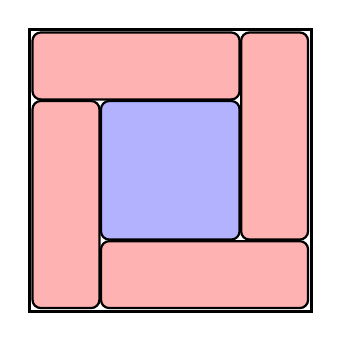
\begin{tikzpicture}[>=latex]
    \def\s{3.5}
    \def\gap{0.85}
    \draw[very thick] (-0.04, -0.04) rectangle (\s + 0.04, \s + 0.04);
    \draw[thick, rounded corners = 3, fill = blue!30] (\gap + 0.02, \gap + 0.02) rectangle
        (\s - \gap - 0.02, \s - \gap - 0.02);
    \draw[thick, rounded corners = 3, fill = red!30] (0, 0) rectangle (\gap, \s - \gap - 0.02);
    \draw[thick, rounded corners = 3, fill = red!30] (0, \s) rectangle (\s - \gap - 0.02, \s - \gap);
    \draw[thick, rounded corners = 3, fill = red!30] (\gap + 0.02, 0) rectangle (\s, \gap);
    \draw[thick, rounded corners = 3, fill = red!30] (\s - \gap, \gap + 0.02) rectangle (\s, \s);
\end{tikzpicture}
 	\caption{}
 	\label{fig:partition-rect}
\end{figure}
	

\subsection{Fooling Set}

Пусть дана матрица некоторой функции. Выберем клетки этой таблицы $a_1, a_2, \ldots, a_n$ так, чтобы
никакие две из них не могли оказаться в одном <<одноцветном>> прямоугольнике, то есть состоящего только
из нулей или только из единиц. Тогда для каждой клетки должен быть свой прямоугольник разбиения. Отсюда
следует, что в дереве протокола должно быть хотя бы $n$ вершин, а высота дерева хотя бы $\log n$. Этот
метод называется \deftext{Fooling Set}.  

Например, его можно применить для функции
$$
    \EQ(x, y) \coloneqq
    \begin{cases}
        1, & x = y,\\
        0, & x \neq y,
    \end{cases}
$$
на строчках длины $m$ мы получим диагональную матрицу $2^m \times 2^m$, и тогда в качестве точек $a_i$
можно выбрать единицы на диагональной матрице. Понятно, что никакие две из них не находятся в одном
одноцветном прямоугольнике. Значит высота коммуникационного дерева хотя бы $\log 2^m = m$.

Похожим образом мы можем доказать нижнюю оценку на функцию $\DISJ(x, y)$ на подмножествах множества
$[n]$, которая принимает значение $1$ тогда и только тогда, когда $ x \cap y = \emptyset$. Для всех
множеств $S \in [2^n]$ рассмотрим ячейку матрицы $a_S \coloneqq (S, \overline{S}$). Заметим, что для $S
\neq S'$ ячейки $a_S$ и $a_{S'}$ не могут лежать в одном прямоугольнике, так как иначе в этом
прямоугольнике лежат ячейки $(S, \overline{S'})$, $(S', \overline{S})$, и в одной из них стоит $0$. Из
чего мы можем заключить, что высота коммуникационного дерева хотя бы $\log 2^n = n$.  


\subsection{Игры Карчмера--Вигдерсона}

\begin{definition}
    \deftext{Формульной сложностью} $L(f)$ формулы $f$ будем называть минимальное возможное число листьев
    дерева, вычисляющего эту формулу (в вершинах дерева стоят булевы операции $\vee, \wedge$, а на
    некоторых рёбрах стоят $\neg $).
\end{definition}

\begin{theorem}[Шеннон]
    Существует такая функция $f\colon \{0, 1\}^n \to \{0, 1\}$, что:
    $$
        L(f) \ge \bigO{\frac{2^n}{n}}.
    $$
\end{theorem}

\begin{proof}
    Заметим, что количество функций $f\colon \{0, 1\}^n \to \{0, 1\}$ равно $2^{2^n}$. Посмотрим на
    всевозможные формулы сложности не более, чем $s$. Каждое из них представляет собой двоичное дерево
    с не более, чем $2s - 1$ вершинами, в которых написаны булевы операции, и не более, чем $s$ листьями,
    в которых написаны переменные. Тогда в каждой вершине стоит один из $n + 6$ символов ($n$ переменных и
    $2$ булевых символа с возможными отрицаниями перед ними), а количество деревьев c не более, чем
    $2s - 1$ вершинами, по теореме Кэли не превосходит:
    $$
        (2s - 1)^{2s - 3}(2s - 1) \le (2s)^{2s} \le 2^{4s \log s}.
    $$ 
    Отсюда следует, что количество деревьев сложности не более, чем $s$, не превосходит
    $2^{4s \log s + 2s \log(n + 6)}$. Осталось убедиться, что при $s < \frac{2^n}{10n}$ количество
    деревьев сложности не более, чем $s$ не превосходит количество функций
    $f\colon \{0, 1\}^n \to \{0, 1\}$. Действительно, при $s < \frac{2^n}{10n}$ верно, что
    $2^{4s\log s + 2s \log(n + 6)} < 2^{2^n}$. А значит существует формула, сложность которой хотя бы
    $\frac{2^n}{10n}$.
\end{proof}
    
На данный момент <<самая сложная>> известная <<явная>>, то есть для неё есть алгоритм, считающий её за
полиномиальное время, функция $f$, для которой выполнено $L(f) \geq n^{3 - \varepsilon}$.

Рассмотрим функцию $f\colon \{0, 1\}^n \to \{0, 1\}$. Для $f$ можно рассмотреть следующую
коммуникационную задачу $\KW_f$: Алиса получает число $x \in f^{-1}(1)$, Боб~--- $y \in f^{-1}(0)$. Их
цель~--- найти хотя бы одну позицию $i$, в которой $x_i \ne y_i$. В случае, если таких битов несколько,
то подойдет любой.

\begin{theorem}[Карчмер--Вигдерсон]
    \label{th:KW-theorem}
    Любую формулу для $f$ можно переделать в коммуникационный протокол для $\KW_f$ с таким же деревом и
    обратно. В частности, минимальная глубина формулы для $f$ равна коммуникационной сложности $\KW_f$.
\end{theorem}

\begin{proof}
    Функцию, которую считает гейт формулы $u$, будем обозначать $f_u$; аналогично, прямоугольник,
    соответствующий вершине протокола $v$, будем обозначать $R_v$.
    
    Начнем с <<простой>> части и построим по формуле коммуникационный протокол. Пусть Алиса получила на
    вход строку $x \in f^{-1}(1)$, а Боб строку $y \in f^{-1}(0)$. Назовём гейт формулы $u$
    \deftext{хорошим}, если $f(x) \neq f(y)$.

    Будем строить протокол, начиная с корня дерева формулы. По условию задачи, корень~--- это хорошая
    вершина, целью Алисы и Боба на каждом раунде будет являться поиск хорошего предка. И тогда,
    перемещаясь на каждом раунде в такого предка, Алиса и Боб найдут хороший лист, в котором и будет тот
    вход формулы, на котором строки Алисы и Боба различаются. Таким образом, для того, чтобы завершить
    доказательство, нам достаточно показать, как найти хорошего предка, передав не более одного
    бита. Рассмотрим текущую вершину $u$ с предками $a, b$ (НУО считаем, что $f_u(x) = 1 \wedge f_u(y) =
    0)$. У нас возможны два случая.
    \begin{enumerate}
        \item В вершине $u$ написан значок $\wedge$. Тогда заметим, что $f_a(x) = f_b(x) = 1$, и при этом
            либо $f_a(y) = 0$, либо $f_b(y) = 0$. Таким образом, Боб может однозначно определить, какой
            из предков является хорошим, и сообщить это Алисе, передав один бит.
        \item В вершине $u$ написан значок $\vee$. Тогда заметим, что $f_a(y) = f_b(y) = 0$, и при этом
            либо $f_a(x) = 1$, либо $f_b(x) = 1$. Таким образом, Алиса может однозначно определить, какой
            из предков является хорошим, и сообщить это Бобу, передав один бит.
    \end{enumerate}


    Теперь по протоколу построим формулу. По индукции, начиная с листьев протокола, для каждой вершины
    протокола $v$ мы предъявим формулу для такой функции $f_v$, что $f_v(X_v) = 1$ и $f_v(Y_v) = 0$,
    где $R_v \coloneqq X_v \times Y_v$.

    Рассмотрим лист протокола $\ell$ и заметим, что прямоугольник $R_{\ell} \coloneqq X_{\ell} \times
    Y_{\ell}$ одноцветный, поэтому все строки $x \in X_{\ell}$ отличаются от всех строк $y \in Y_{\ell}$
    в какой-то фиксированной позиции $i_{\ell}$, в частности это означает, что выполнен один из двух
    следующих случаев:
    \begin{itemize}
        \item для всех $x \in X_{\ell}, y \in Y_{\ell}$ бит $x_{i_{\ell}} = 1$ и $y_{i_{\ell}} = 0$,
            тогда мы можем определить $f_{\ell} \coloneqq x_{i_{\ell}}$;
        \item для всех $x \in X_{\ell}, y \in Y_{\ell}$ бит $x_{i_{\ell}} = 0$ и $y_{i_{\ell}} = 1$,
            тогда мы можем определить $f_{\ell} \coloneqq \neg x_{i_{\ell}}$.
    \end{itemize}
    Других случаев не существует, поскольку если найдутся такие $x, x' \in X$, что $x_{i_{\ell}} \neq
    x'_{i_{\ell}}$, то они одновременно не могут отличаться в позиции $i_l$ ни от какого $y$ (случай
    $y_{i_{\ell}} \neq y'_{i_{\ell}}$ аналогичен).

    Построим теперь формулу для функции $f_v$, если у нас уже есть формулы для функций $f_a$ и $f_b$, где
    $a, b$~--- потомки вершины $v$. Заметим, что прямоугольники $R_a$ и $R_b$ получены рассечением
    прямоугольника $R_v$ на две части либо вертикальным, либо горизонтальным сечением. Рассмотрим эти
    случай отдельно и заметим, что:
    \begin{itemize}
        \item если сечение было горизонтальным, то $Y_a = Y_b = Y_v$ и $X_v = X_a \cup X_b$ и в таком
            случае нам подойдет формула $f_v \coloneqq f_a \vee f_b$;
        \item если сечение было вертикальным, то $X_a = X_b = X_v$ и $Y_v = Y_a \cup Y_b$ и в таком
            случае нам подойдет формула $f_v \coloneqq f_a \wedge f_b$.
    \end{itemize}
\end{proof}
    \subsection{Применения теории информации в коммуникационной сложности}

Начнем с урезанной коммуникационной модели. Определим функцию индексирования:
$$
    \Ind\colon [n] \times \{0,1\}^n \to \{0, 1\},\qquad \Ind(x, y) = y_x,
$$ 
где $y_x$~--- $x$-ый бит числа $y$. Рассмотрим следующую коммуникационную задачу, в которой Алиса
получает на вход число $x \in [n]$, а Боб получает $y \in \{0,1\}^n$. Им нужно найти
$\Ind(x, y)$. Нетрудно показать, что коммуникационная сложность этой задачи равна $\bigO{\log n}$, так как
Алиса может послать $x$, и по $x$ Боб может сказать бит, стоящий в $x$-ой позиции.

Усложним задачу. Пусть биты может посылать только Боб. Тогда коммуникационная сложность этой задачи
становится $\bigO{n}$, так как в итоге Боб должен послать информацию про все биты своего числа. Иначе у
Алисы может быть бит $x$, про который она ничего не знает.

Будем теперь считать, что Алиса и Боб получают входы согласно равномерному распределению среди всех
возможных входов. Посылать информацию может только Боб. Но теперь Бобу с Алисой разрешено делать ошибку
$\varepsilon \coloneqq \frac{1}{2} - \delta$, то есть не больше, чем на $\varepsilon \abs{X \times Y}$
входах можно сделать ошибку. Докажем, что коммуникационная сложность этой задачи равна
$\bigO{\delta^2 n}$. 

Рассмотрим коммуникационный протокол $\pi$, решающий нашу задачу. Заметим, что $\DCC^1(\pi) \ge \log
\abs{M}$, где $M$~--- множество листьев, а $\DCC^1$~--- коммуникационная сложность задачи, в 
которой только Боб может посылать биты. Рассмотрим энтропию $h(M)$ распределения на листьях, которая 
получается естественным способом из распределения на входах. Тогда нетрудно получить следующие
неравенства: 
$$
    \log{\abs{M}} \ge h(M) \ge I(M:y).
$$ 
По \textit{chain rule} мы получаем, что:
\begin{align*}
    I(M:y) &= \sum_i I(M:y_i \mid y_{x_{< i}})\\
           &= \sum_i h(y_i \mid y_{x_{< i}}) - h(y_i \mid M, y_{x_{\le i}})\\
           &= \sum_i h(y_i) - h(y_i \mid M, y_{x < i}) & \text{так как все $y_i$ независимы}\\
           &\ge \sum_i h(y_i) - h(y_i \mid M)\\
           &\ge \sum_i I(M : y_i).
\end{align*}

Для оценки $I(M : y_i)$ нам потребуется вспомогательная величина. Пусть $r_i^m$~--- вероятность
ошибки, при условии того, что Боб послал сообщение $m$ и $x = i$. Из определения $r_i^m$ следует, что
$\Exp\limits_{i, m}[r_i^m] \le \frac{1}{2} - \delta$.

Интуиция, скрывающаяся за следующими действиями такова: если $I(M : y_i)$ малая величина, то
сообщение Боба <<почти ничего>> не сообщает об $i$-ом бите и, как следствие, если у Алисы $x = i$, мы
получим ошибку с вероятностью примерно $\frac{1}{2}$. Попробуем формализовать эту стратегию.
\begin{align*}
  I(M : y_i) &= h(y_i) - h(y_i \mid M)\\
           &= 1 - h(y_i \mid M) & \text{поскольку распределение равномерное}\\
           &= 1 - \Exp_m[h(y_i \mid M = m)]\\
           &= 1 - \Exp_m[h(y_i \mid M = m, x = i)] & \text{$y_i$ и $M$ независимы относительно $x$}\\
           &= 1 - \Exp_m[h(r^m_i)].
\end{align*}
Теперь попробуем оценить всю сумму:
\begin{align*}
  \sum_i I(M : y_i) &= \sum_i 1 - \Exp_m[h(r^m_i)]\ge & \text{неравенство Йенсена}\\
                  &\ge \sum_i 1 - h\left(\Exp_m[r^m_i]\right) \\
                  &= n - n \sum_i\frac{1}{n} h\left(\Exp_m[r_i^m]\right) \ge & \text{неравенство Йенсена} \\
                  &\ge n - n h\left(\Exp_{i, m}[r_i^m]\right) \\
                  &\ge n \left(1 - h \left(\frac{1}{2} - \delta\right)\right)\\
                  &= \Omega(\delta^2n).
\end{align*}

Похожих идей будем придерживаться и в случае обычных коммуникационных протоколов.

\begin{definition}
    Пусть $f\colon X \times Y \to Z$ и $\mu$~--- распределение на $X \times Y$. Заметим, что для любого
    коммуникационного протокола $\Pi$ для функции $f$ распределение $\mu$ индуцирует распределение на
    листьях данного протокола естественным образом. \deftext{Внешней информационной стоимостью} (или 
    \deftext{внешним информационным разглашением}) протокола $\Pi$ по распределению $\mu$ будем называть
    величину:
    $$
        \ICext[\mu](\Pi) \coloneqq I(\Pi(X, Y) : X, Y).
    $$
    Также определим внешнюю информационную сложность самой функции
    $\ICext[\mu](f) \coloneqq \min\limits_{\Pi} \ICext[\mu](\Pi)$.

    По аналогии мы может рассмотреть и \deftext{внутреннее информационное разшлашение} (или 
    \deftext{внутренюю информационную стоимость}).
    $$
        \ICint[\mu](\Pi) \coloneqq I(\Pi(X, Y) : X \mid Y) + I(\Pi(X, Y) : Y \mid X).
    $$
\end{definition}

Следующая теорема на дает связь между коммуникационной сложностью и новой метод сложности.

\begin{theorem}
    Пусть $\pi$~--- протокол некоторой коммуникационной задачи c мерой $\mu$ на входах. Тогда:
    $$
        \DCC(\pi) \ge \ICext[\mu](\pi) \ge \ICint[\mu](\pi).
    $$ 
\end{theorem}

\begin{proof}
    $\DCC(\pi) \ge \log(M) \ge h(\pi) \ge I(\pi : X, Y)$, где $h(\pi)$~--- энтропия от распределения на
    листьях. Откуда следует первое неравенство.
    
    Теперь докажем второе: $I(\pi : X, Y) \ge I(\pi : X \mid Y) + I(\pi : Y \mid X)$. По chain rule мы
    получаем, что $I(\pi : X, Y) = \sum\limits_i I(\pi_i : X, Y \mid \pi_{< i})$, где $\pi_i$~--- это
    случайная величина, соответствующая $i$-ому биту, переданному в протоколе. Мы хотим показать, что:
    $$
        I(\pi_i : X, Y \mid \pi_{< i}) \ge I(\pi_i : X \mid Y, \pi_{< i}) +
        I(\pi_i : Y \mid X, \pi_{< i}),
    $$

    Для доказательства мы заметим, что:
    \begin{align*}
      I(\pi_i : X, Y \mid \pi_{< i}) &\ge I(\pi_i : X \mid Y, \pi_{< i}) \\
      I(\pi_i : X, Y \mid \pi_{< i}) &\ge I(\pi_i : Y \mid X, \pi_{< i})
    \end{align*}
    Так как по $\pi_{< i}$ мы знаем в какой вершине протокола мы находимся после $i$ шагов, то в этой
    вершине либо Алиса либо Боб посылают бит и $\pi_i$ будет определяться однозначно либо по $X$, либо по
    $Y$. Откуда следует, что одна из величин $I(\pi_i : X \mid Y, \pi_{< i})$, $I(\pi_i : Y \mid X,
    \pi_{< i})$ равна $0$. А поскольку $I(\pi_i : X, Y \mid \pi_{< i})$ не меньше второй величины, то мы
    получили требуемое неравенство.

    По chain rule получаем, что:
    $$
        \sum I(\pi_i : X \mid Y, \pi_{< i}) + I(\pi_i : Y \mid X, \pi_{< i}) =
        I(\pi : X \mid Y) + I(\pi : Y \mid X).
    $$ 
    Окуда следует второе неравенство из условия теоремы.
\end{proof}

При этом  для любого протокола $\pi$ существует такая мера $\mu$, что $\log \abs{\pi} = \ICext[\mu](\pi)$,
где $L$~--- число листье в протоколе.

\begin{theorem}[Храпченко]
    $L(\oplus_n) \ge \bigO{n^2}$, где функция $\oplus_n$ равна чётности количества единиц в записи числа
    длины $n$.
\end{theorem}

\begin{proof}
    Рассмотрим $\KW_{\oplus_n}$. Покажем, что $\ICint[\mu](\KW_{\oplus_n}) \ge 2 \log n$, откуда будет
    следовать, что $\DCC(\oplus_n) \ge 2 \log n$ и по теореме \ref{th:KW-theorem} мы получим $L(\oplus_n)
    \ge n^2$.

    Определим распределение $\mu$: равномерное распределение на парах $(x, x \oplus e_i) $, по всем $x
    \in \oplus_n^{-1}(1)$ (по всем $x$, в записи которых нечётное число единиц). Тогда:
    \begin{align*}
        I(\pi : Y \mid X) &= I(\pi: x \oplus e_I \mid X) = I(\pi : e_I \mid X) = h(e_I \mid X) - h(\pi
                            \mid X, e_I) \\
        &= h(e_I \mid X) = h(e_I) = \log n.
    \end{align*}
    Аналогично со вторым слагаемым.
\end{proof}

Данная оценка является точной.

    \section{Колмогоровская сложность}

\begin{definition}
    Пусть $F\colon \{0, 1\}^{*} \to \{0, 1\}^{*}$~--- вычислимая функция. \deftext{Сложностью описания}
    $x$ относительно  функции $F$ мы будем называть:
    $$
        \Kolm_F(x) = \min\{\abs{p} : F(p) = x\}.
    $$ 
    Если такого $p$ не найдётся, то $\Kolm_F(x) = +\infty$.
    
    Будем говорить, что способ описания $F$ \deftext{не хуже} способа описания $G$, и обозначать $F \prec
    G$ если существует такая константа $c_{FG}$, что для любого $x$ выполнено:
    $$
        \Kolm_F(x) \le \Kolm_G(x) + c_{FG}.
    $$

    Будем называть способ описания \deftext{оптимальным}, если он не хуже любого другого способа
    описания.
\end{definition}

\begin{theorem}
    Существует оптимальный способ описания.
\end{theorem}

\begin{proof}
    Доказательство оставим в качестве упражнения.
\end{proof}

Если $F, G$~--- оптимальные способы описания, то $\abs{\Kolm_F(x) - \Kolm_G(x)} \le c_{FG}$ для всех $x$
и некоторой константы $c_{FG}$.

\begin{definition}
    Будем называть \deftext{колмогоровской сложностью} $x$ число $\Kolm(x) \coloneqq \Kolm_u(x)$, где
    $u$~--- какой-то оптимальный способ описания.
\end{definition}

Мы не уточнили, какой из оптимальных способов описания рассматриваем, как следствие это означает, что мы
определили колмогоровскую сложность с точностью до аддитивной константы. Поэтому говорить о сложности
одной строки не имеет смысла (действительно, если взять конкретную строку $w$, то у нас существует
алгоритм, в тексте которого уже присутствует эта строка $w$, и он выписывает её на пустом входе). 
Чтобы данное определение обрело смысл, мы будем иметь ввиду, что у нас есть семейство строк,
параметризованное каким-либо параметром (чаще всего $n$).

Рассмотрим нетокоры простые свойства колмогоровской сложности.

\begin{enumerate}
    \item $K(x) \le |x| + c$;
    \item $K(xx) \le |x| + c$;
    \item если в слове $x$ длины $n$ не более $np$ единиц, то
        $$
            \Kolm(x) \le \entropy(p) n + \bigO{1},
        $$ 
        где $\entropy(p)$~--- энтропия нечестной монетки, выпадающей орлом с вероятностью $p$, где $0 \le
        p \le 1$.
\end{enumerate}

Первое и второе утверждения следуют и того, что существует алгоритм, копирующий свой вход на выходную
ленту, а также алгоритм, который делает это дважды.

Рассмотрим множество $S$, состоящее их всех слов длины $n$, в которых не более $pn$ единиц. Заметим, что
$x \in S$, и его можно описать при помощи номера в этом множестве (подойдёт любая нумерация
элементов). Осталось заметить, что:
$$
    |S| \le \sum_{k = 1}^{np} \binom{n}{k} \leq 2^{\entropy(p) n},
$$
где последнее неравенство следует из утверждения \ref{prop:binomial-coef}.


\begin{theorem}
    Рассмотрим такую всюду определенную функцию $M\colon \{0, 1\}^{*} \to \mathbb{N}$, что для любого $x
    \in \{0, 1\}^{*}$ верно $M(x) \le \Kolm(x)$. Если для любой константы $c$ существует такое
    $w \in \{0, 1\}^{*}$, что $M(w) > c$, то $M$~--- невычислима.
\end{theorem}

Хотим провести рассуждения, аналогичные рассуждениям в \textit{парадоксе Бэрри}: рассмотрим выражение
<<Наименьшее натуральное число, которое нельзя описать менее чем одиннадцатью русскими
словами>>. Поскольку слов конечное число, существует конечное множество фраз из менее чем одиннадцати
слов, и, следовательно, конечное подмножество натуральных чисел, определяемых фразой из одиннадцати
слов. Однако множество натуральных чисел бесконечно, следовательно, существуют числа, которые нельзя
определить фразой из менее чем одиннадцати слов. Среди них, существует наименьшее натуральное число
(наименьшее число можно выбрать из любого подмножества натуральных чисел), <<не описываемое менее чем
одиннадцатью словами>>. Но именно это число определяется приведённой выше фразой, и в ней менее
одиннадцати слов, а значит, оно не может являться искомым наименьшим числом и не может описываться данной
фразой. Возникает парадокс: должно существовать число, описываемое данной фразой, но поскольку выражение
само себе противоречит, не может существовать числа, им описываемого.
    
\begin{proof}
    Рассмотрим первое слово $x_c$, для которого выполняется условие $M(x_c) \ge c$ для некоторой
    константы $c$. Определим функцию $F(\overline{c}) = x_c,$ где $\overline{c}$~--- битовая запись числа
    $c$. Заметим, что если $M$ вычислима, то и функция $F$ будет вычислимой. Но тогда $\Kolm(x_c) \le
    \log c + c_0$, поскольку $\abs{\overline{c}} = \log c$, и мы получаем противоречие, так как
    $M(x_c) = c > \log c = \Kolm(x_c)$. 
\end{proof}

\begin{corollary}
    Любой оптимальный способ определим не всюду.
\end{corollary}

\begin{theorem}
    \label{th:99-words}
    $99\%$ слов $x \in \{0, 1\}^n$ имеют сложность $n - \bigO{1}$. 
\end{theorem}

\begin{proof}
    Зафиксируем какой-то оптимальный способ описания $U$. Тогда число описаний длины не более $n - c$ не
    превосходит $2^{n - c + 1}$. Тогда у хотя бы $2^{n} - 2^{n - c + 1}$ длина кратчайшего описания не
    менее $n - c + 1$, откуда нетрудно получить утверждение теоремы.
\end{proof}


\subsection{Условная колмогоровская сложность}

Рассмотрим вычислимую функцию $F(p, y) = x$. Будем говорить, что
\deftext{сложность описания $x$ относительно функции $F$ при условии $y$} равна 
$$
    \Kolm_F(x \mid y) = \min\{\abs{p} : F(p, y) = x \}.
$$ 

\begin{theorem}
    Для любого $y$ существует оптимальный способ описания.
\end{theorem}

\begin{definition}
    Определим колмогоровскую сложность $\Kolm(x \mid y) = \Kolm_u(x \mid y)$ для некоторого оптимального
    способа описания $u$ при фиксированном $y$.
\end{definition}

Для условной колмогоровской сложности выполнены естественные свойства:
\begin{itemize}
    \item $\Kolm(x \mid y) < \Kolm(x) + \bigO{1}$;
    \item $\Kolm(f(x) \mid x) = \bigO{1}$ для любой вычислимой функции $f$.
\end{itemize}

\begin{definition}
    Определим колмогоровскую сложность пары $\Kolm(x, y) = \Kolm(\avg{x, y})$, где $\avg{x, y}$ ---
    фиксированная кодировка.
\end{definition}

Для энтропии мы знаем, что $\entropy(x, y) = \entropy(x) + \entropy(y \mid x)$. Хочется доказать
аналогичное утверждение про колмогоровскую сложность. Равенство для колмогоровской сложности не всегда
верно. Также неверно следующее неравенство:  
$$
    \Kolm(x, y) \le \Kolm(x) + \Kolm(y \mid x) + \bigO{1}.
$$
    
Это можно видеть из следующего примера.
\begin{example}
    Рассмотрим пары $(x, y)$, для которых $|x| + |y| = n$. Таких пар $n \cdot 2^n$. Аналогично
    доказательству теоремы \ref{th:99-words} найдётся пара сложности $n + \log n - \bigO{1}$. Тогда для
    неё мы получим, что  
    $$
        \Kolm(x, y) = \Kolm(x) + \Kolm(y \mid x) + \log n + \bigO{1}.
    $$
\end{example}

Мы момжет чуть-чуть поправить неравенство, чтобы оно стало верным.
\begin{theorem}
    $$
        \Kolm(x, y) \le \Kolm(x) + \Kolm(y \mid x) + \bigO{\log \Kolm(x, y)}.
    $$
\end{theorem}

\begin{proof}
    Пусть $n = n_1n_2\ldots n_k$~--- длина описания $x$. Тогда пару $\avg{x, y}$ можно закодировать
    числом:
    $$
        n_1n_1n_2n_2 \ldots n_kn_k01\{\text{описание } x\}\{\text{описание } y \text{ при известном $x$}\}.
    $$
    Что дает нам описание $(x, y)$ длины $\Kolm(x) + \Kolm(y \mid x) + \bigO{\log \Kolm(x, y)}$.
\end{proof}

\begin{theorem}[Колмогоров--Левин]
    Имеет место равенство 
    $$
        \Kolm(x, y) = \Kolm(x) + \Kolm(y \mid x) + \bigO{\log \Kolm(x, y)}.
    $$
\end{theorem}

\begin{proof}
    Неравенство в одну сторону мы показали. Докажем неравенство в другую сторону.
    
    Положим $n \coloneqq \Kolm(x, y)$. Определим множество $S \coloneqq \{(a, b) \mid \Kolm(a, b) \le n
    \}$. Будем рассматривать сечение $S_{x}$. Пусть $\log \abs{S_x} = m$. Тогда для описания $y$ по $x$
    нам нужно перечислить элементы $S_x$ и найти $y$. Для этого нам нужно знать $n$, это потребует
    $\bigO{\log n}$  битов, и нужно уметь перечислять элементы $S_x$, для этого нам потребуется $m$
    битов. Тогда:
    $$
        \Kolm(y \mid x) \le m + \bigO{\log n}.
    $$ 
    Для описания $x$ рассмотрим все такие $t$, что $\log \abs{S_t} \ge m$, и выберем из них $x$. Для
    этого нам опять потребуется $\log n$ битов, для хранения $n$, и $n - m$ битов для перечисления $t$,
    так как таких $t$ не больше, чем $\frac{\abs{S}}{2^m} \le 2^{n + 1 - m}$, так как $\abs{S} \le
    2^{n + 1}$. Откуда:
    $$
        \Kolm(x) \le n - m + \bigO{\log n}.
    $$ 
    Тогда получаем:
    $$
        \Kolm(x) + \Kolm(y \mid x) \le n + \bigO{\log n} = \Kolm(x, y) + \bigO{\log \Kolm(x, y)}
    $$
\end{proof}

Можно определить $I_{\Kolm}(x: y) = \Kolm(y) - \Kolm(y \mid x)$. Также верно неравенство 
$$
    \abs{I_{\Kolm}(x : y) - I_{\Kolm}(y : x)} \le \log \Kolm(x, y) + \bigO{1}.
$$ 
От логарифма избавиться не получится, можно рассмотреть такой $x \in \{0, 1\}^n$, что $\Kolm(x \mid n) =
n - \bigO{1}$. Тогда $I_{\Kolm}(n : x) = \bigO{1}$, а $I_{\Kolm}(x : n) = \log n$. 
    \section{Применения колмогоровской сложности}

Колмогоровская сложность применяется в задачах, связанных с попытками доказать или опровергнуть
$\mathrm{NP}$-полноту задачи $\lang{MCSP}$, в которой по таблице истинности функции $f\colon \{0, 1\}^n
\to \{0, 1\}$ и числу $s < 2^n$ необходимо определить, существует ли булева схема размера $s$, которая
считает данную функцию. Нетрудно понять, что эта задача принадлежит классу $\NP$. Но не доказано,
является ли эта задача $\NP$-полной.  

Рассмотрим более простую задачу. Обозначим за $L_k$ множество языков, принимаемых детерминированными
автоматами с одной лентой и $k$ головками на ней, причём головки едут только в одну сторону. 

\begin{proposition}
    $L_{k + 1} \nsubseteq L_{k}$.
\end{proposition}

\begin{proof}
    Рассмотрим язык $L$, состоящий из строк вида:
    $$
        w_1\#w_2\#\ldots \#w_{m - 1}\#w_m\#w_m\#w_{m - 1}\#\ldots \#w_2\#w_1,
    $$
    где $m$~--- фиксировано, а $w_i$~--- произвольные слова. Покажем, что если $m > \frac{k(k - 1)}{2}$,
    то язык $L$ не распознаётся автоматом с $k$ головками, а если это не так, то распознаётся.
    
    В каждом слове языка $L$ есть по два слова $w_i$. Будем называть их <<левым>> и <<правым>>
    соответственно. Пусть $m \leq \frac{k(k - 1)}{2}$. Опишем автомат с $k$ головками, который распознаёт
    язык $L$. Сначала все $k$ головок расположены на началах левых слов $w_1, w_2, \ldots,
    w_k$. Следующим действием последняя головка, которая стоит в начале $w_k$, доходит до начала правого
    слова $w_{k - 1}$. Далее проверяем равенство левых и правых слов $w_i$, где $1 \leq i \leq k -
    1$. Тем самым, <<потратив>> одну головку мы проверили равенство $k - 1$ слова сначала и с
    конца. Далее повторяем алгоритм для $k - 1$ головки и слова, без первых и последних $k - 1$ слов
    $w_i$. Тем самым мы проверим $(k - 1) + (k - 2) + \ldots + 1 = \frac{k(k - 1)}{2}$ слов. 
    
    Пусть теперь $m > \frac{k(k - 1)}{2}$. Посмотрим на левый и правый блоки с номером $\ell$ (слово
    $w_{\ell}$). Пусть в какой-то момент головки $i$ и $j$ стоят на разных копиях слова $w_l$. Тогда эта
    пара головок $(i, j)$ ни в какой другой момент времени не будет находиться в одинаковых словах $w_r$,
    при $r \neq \ell$, так как головки движутся только вправо. Тогда, так как $m > \frac{k(k - 1)}{2}$,
    то для какого-то слова $w_{\ell}$ верно, что в каждый момент времени только в одной копии $w_{\ell}$ может
    находиться головка. 
    
    Построим протокол, который будет запоминать состояния автомата и позиции головок для каждого такого
    момента, что либо какая-то головка оказалась в слове $w_{\ell}$, либо какая-то головка покинула слово
    $w_{\ell}$. Попробуем восстановить $w_{\ell}$ по протоколу. Подставим $x$ на место $w_{\ell}$. Если
    автомат выдал такой же протокол работы, то $x$ потенциально подходит. Предположим, что нашлось $2$
    подходящих слова $x$ и $y$, для которых протокол работает правильно. Тогда рассмотрим слово
    $w_{x, y}$, равное слову $w$, в котором левое слово $w_{\ell}$ заменили на $x$, а правое слово
    $w_{\ell}$ заменили на $y$. Заметим, что для слов $w$ и $w_{x, y}$ алгоритм работает одинаково. А
    значит $w_{x, y}$ лежит в нашем языке, что не правда. Откуда получаем противоречие, а значит по
    протоколу мы однозначно восстанавливаем $w_{\ell}$.
    
    Пусть длина слова $w$ равна $n$, и в нём зафиксированы слова $w_i, i \neq {\ell}$. Тогда размер
    протокола для $w$ равен $\bigO{k^3 \log n}$, где $k$~--- число головок. Осталось заметить, что 
    символов для кодирования строки $w$, с фиксированными $w_i, i \neq {\ell}$, не меньше, чем
    $\sum\limits_{i \neq \ell}{\abs{w_i}} + \bigO{k^3 \log n}$. Заметим, что существуют такие $w_i$, что
    $\abs{w_i} = s$ для любого $i$ и $K(w_1\#\ldots\#w_m\#w_m\#\ldots\#w_1) \geq ms - c$. Но из
    предыдущих рассуждений мы получили, что колмогоровская сложность $w$ равна $(m - 1)s +
    \bigO{\log s}$, так как $\sum\limits_{i \neq l} {\abs{w_i}} = (m - 1)s$. Тогда при больших $s$ мы
    получаем противоречие. А значит язык $L$ не лежит в $L_k$, теорема доказана.    
\end{proof}


\section{Случайные по Мартин-Лёфу}

Рассмотрим бесконечную строчку $w = x_1x_2x_3\ldots $ Хотим узнать, случайна ли эта строчка, или она
получена каким-то алгоритмом. Предположим, что мы знаем биты $x_1, x_2, \ldots, x_{n - 1}$. Можно ли узнать
бит $x_n$? Если бы можно было узнать все биты $x_n$ по предыдущим, то понятно, что строка не
случайная. Но как часто можно узнавать следующий бит по предыдущим в случайной строке? 

Хотелось бы сказать, что строка случайная, если существует такая константа $c$, что для любого $n$ верно
$\Kolm(x_{\leq n}) \geq n - c$ (то есть когда колмогоровская сложность достаточно большая). Оказывается,
что не существует такой последовательности $x_i$, для которой это неравенство выполнено.
\begin{theorem}
   Для любой последовательности $x_1x_2x_3\ldots$ и числа $n_0$ найдётся такое $n > n_0$, что
   $\Kolm(x_{\leq n}) \le n - \bigO{\log n}$. В частности, для любой константы $c$ найдётся такое $n$,
   что $\Kolm(x_{\leq n}) \le n - c$. 
\end{theorem}

\begin{proof}
    Рассмотрим любую последовательность $x_1x_2x_3\ldots$ и её префиксы $x_1\ldots x_kx_{k + 1}\ldots
    x_{k + m}, $ где $k + m = n$. Рассмотрим префиксы длины $n$, которые разбиваются на две части,
    $x_1\ldots x_k$ и $x_{k + 1} \ldots x_n$, причём $1x_1x_2\ldots x_k = m$ (не все $n$ подходят). Тогда
    $\Kolm(x_{\leq m + k}) \leq m + \bigO{1}$, так как зная последние $m$ символов префикса длины $n$ мы можем
    восстановить весь префикс. Но длина всего префикса равна $n = m + \log m$, откуда получаем, что
    $\Kolm(x_{\leq n}) \leq n - \bigO{\log n}$. Осталось заметить, что $n$ можно выбрать сколь угодно большое,
    что и доказывает теорему.
\end{proof}


\begin{definition}
    Функцию $F$ будем называть \deftext{беспрефиксной}, если из того, что $F$ определена на $x$ и $y$
    следует, что $x$ не является префиксом $y$, и наоборот.
\end{definition}

Для беспрефиксных функций можно определить понятие колмогоровской сложности так же, как и для обычных
функций. Мы будем обозначать её через $\KolmP(x)$.

\begin{definition}
   Строку $w$ будем называть \deftext{случайной}, если существует такая константа $c$, что
   $\KolmP(w_{\leq n}) \ge n - c$ для всех $n \in \mathbb{N}$.
\end{definition}

В определении колмогоровской сложности мы пользовались тем, что существует оптимальный способ описания
для беспрефиксных функций. Докажем это в следующей теореме.

\begin{theorem}
    Существует оптимальный беспрефиксный способ описания.
\end{theorem}

Для доказатетельства данной теоремы нам понадобится вспомогательное утверждение.

\begin{theorem}
    Cуществует такой алгоритм $A$, что для любой вычислимой функции $F$ выполняются условия:
    \begin{itemize}
        \item если $ F $ --- беспрефиксная, то $ A(F) = F $;
        \item если $ F $ --- не беспрефиксная, то $ A(F) = F' $, где $F'$ --- беспрефиксная.
    \end{itemize}
\end{theorem}

\begin{proof}
    Пусть на вход дана функция $F$, и мы хотим посчитать $F(x)$. Запустис $F$ параллельно на всех входах
    (стандартная операция из теории вычислимости). Если в какой-то момент, до того, как мы посчитали
    $F(x)$ оказалось, что алгоритм подсчета $F$ остановился двух строках $y$ и $yz$ для некоторых $y$ и
    $z$, то зацикливается. Иначе выдаем значение $F(x)$.

    Заметим, что если алгоритму $A$ дали на вход беспрефикснцю функцию, то алгоритм $A$ выдает ее же, и
    $A$ всегда выдаёт какую-то беспрефиксную функцию.
\end{proof}

\begin{proof}
    В качестве оптимального способа описания мы можем использовать $U'(x, y) \coloneqq A(x(y))$, где $(x,
    y)$ задано беспрефиксным образом, например все биты $x$ удваиваются, затем идет $01$, а затем
    кодировка $y$.
\end{proof}

Заметим, что $\KolmP(x) \le \Kolm(x) + 2 \log \Kolm(x) + \bigO{1}$. Чтобы доказать это неравенство
применим кодировку: $p \to a_1a_1a_2a_2 \ldots a_ka_k01p$, где $p$~--- описание $x$ и $\abs{p} =
a_1a_2\ldots a_k$. Тогда $k \leq \log \Kolm(x)$ и $\KolmP(x) \le \Kolm(x) + 2\log \Kolm(x) +
\bigO{1}$.

\begin{theorem}
    Мера Бернулли неслучайных последовательностей равна $0$. 
\end{theorem}

\begin{proof}
    Рассмотрим некоторую неслучайную последовательность $x_1x_2\ldots$. Тогда так как она не случайна, то
    для любого $c$ существуют $n_1,n_2, \ldots,n_l, \ldots$, что $\KolmP(x_{\leq n_i)} \leq n_i -
    c$. Тогда
    $$
        \sum\limits_{\{x \mid \KolmP(x) \le n - c, \abs{x} = n\}} 2^{-n} \leq
        \sum_x 2^{-\KolmP(x) - c} \le 2^{-c} \cdot \sum_x 2^{-\KolmP(x)} \le 2^{-c}.
    $$
    Последнее неравенство верно, так как код префиксный, и можно применить неравенство
    Крафта--Макмиллана. Также если $A_i$~--- множество строк с плохими префиксами $x_1x_2\ldots x_i$, то
    мера Бернулли неслучайных последовательностей
    $$
        M\left(\bigcup A_i\right) \leq \sum_{\{x \mid \KolmP(x) \le n - c\}} 2^{-n} < 2^{-c}.
    $$
    Осталось устремить $c$ к бесконечности, и получить требуемое.    
\end{proof}

\begin{theorem}[Закон больших чисел в форме Харди--Литлвуда]
    Для почти всех последовательностей $x \coloneqq  x_1x_2 \dots x_n \dots$ (с вероятностью $1$)
    выполнено:
    $$
        \left|\frac{x_1 + x_2 + \dots + x_n}{n} - \frac{1}{2}\right| =
        \bigO{\sqrt{\frac{\log n}{n}}}. 
    $$
\end{theorem}

\begin{proof}
    Пусть в $x_1 \dots x_n$ всего $p_n \cdot n$ единиц и $(1 - p_n) \cdot n$ нулей.
    $$
        \KolmP(x_1 \dots x_n) \le \Kolm(x_1 \dots x_n) + \bigO{\log n} \le h(p) \cdot n + \bigO{\log n}.
    $$

    
    Пусть $p \coloneqq \frac{1}{2} + \delta_n$. Разложим $h(p)$ в ряд в окрестности $\frac{1}{2}$:
    $$ 
        h(1 / 2 + \delta_n) \cdot n = (1 - c_H \cdot \delta_n^2 + o(\delta_n^2)) \cdot n \le
        (1 - c'_H \cdot \delta_n^2) \cdot n.
    $$
    Таким образом для случайной последовательности (т.е. с вероятностью 1):
    $$
        n - c \le \KolmP(x_1 \dots x_n) \le n - c'_H \cdot \delta_n^2 \cdot n + \bigO{\log n}.
    $$

    Получаем, что $\delta_n^2 \le \bigO{\frac{\log n}{n}}$.
\end{proof}

    \selectlanguage{english}
    \printbibliography[title = \foreignlanguage{russian}{Список литературы}]
\end{document}